\chapter{Segregated Runge-Kutta time integration schemes}
\label{chap-SRK}

\section{Introduction}
\label{sec-C6_introduction}

Many problems in science and engineering can be simulated by incompressible flow solvers, e.g., flows around aircrafts during take-off and landing, cars, bridges, wind turbines, etc. Incompressible flows are also encountered when simulating liquid metal blankets in fusion reactors or blood flow in bio-mechanics. The increasing computer power of super-computers has motivated the interest in high-fidelity massively parallel predictive tools on unstructured meshes for this type of applications. Higher levels of accuracy in space can be based on refined meshes or higher-order approximations, being the use of hp-adaptive simulations the most refined approach so far.

The transient incompressible Navier-Stokes system of partial differential equations is nonlinear (due to convection) and indefinite (due to the divergence-free constraint), which complicates its discretization and the linear solver step. A fully implicit time-integration involves nonlinear iterations at every time step, increasing computational cost. On the other hand, it is hard to define scalable parallel solvers for non-symmetric and indefinite problems. The definition of scalable preconditioners for this nonlinear system of equations is an open problem both for domain decomposition and multigrid techniques. 
Further, the nonlinear nature of the problem requires frequent preconditioner set-up steps, that make this approach computationally intensive. 

The velocity-pressure block-segregation can be understood as a solver (introducing an additional splitting error) instead of a preconditioner, leading to the popular pressure-correction or fractional-step methods \cite{kim_application_1985,le_improvement_1991,codina_pressure_2006,badia_algebraic_2008}. This approach involves to solve decoupled a momentum equation for the velocity and a pressure Poisson equation. This is the most popular approach for the simulation of turbulent incompressible flows. The time integration of the momentum equation can be carried out using explicit, semi-implicit, or fully implicit methods. The fully implicit method has some of the drawbacks considered above, whereas an explicit integration of the viscous terms is not suitable for wall-bounded flows. In order to capture the viscous effects around solids, very refined anisotropic meshes are required, leading to too stringent viscous Courant-Friedrichs-Lewy (CFL) conditions. The use of hp-adaptivity makes hard to use explicit methods, since intensive local refinement in some parts, e.g., the tip of an airfoil, leads to global time steps that must go to zero as $\frac{h^2 }{p^4}$ for stability purposes, being $h$ the characteristic element size and $p$ the degree of interpolation, and local time-stepping cannot be efficiently exploited on parallel platforms. The use of semi-implicit methods, which treat implicitly the diffusive term and explicitly the convective one, seems to be the perfect compromise for turbulent flows around objects and viscous flows. The time step restriction is given by the convective {CFL} condition, which is much weaker than the diffusive one and also avoids nonlinear iterations. In fact, the majority of direct and large eddy simulations of incompressible flows involve semi-implicit methods, in which only the viscous term is treated implicitly. 

When high-order time integration aims to be achieved, a popular approach is to use Runge-Kutta (RK) schemes, due to the good stability properties, high-order accuracy, and the easy computation of time error estimates for adaptive time stepping (see \cite{hairer_numerical_1989,de_swart_construction_1997}). RK schemes involve several systems of equations at each time step. Further, when we use an implicit scheme all stages can be coupled, resulting in a large system of equations to be solved, which is quite impractical in terms of CPU cost. This is the case of \cite{sanderse_energy-conserving_2013}, where energy-conserving implicit Runge-Kutta methods are investigated. 
This drawback can be bypassed using an explicit scheme, with the problems related by the time step restriction to ensure stability. An accuracy analysis of these methods is done by Sanderse et al in \cite{sanderse_accuracy_2012}. 
Diagonally Implicit RK methods (DIRK) can be used to avoid stability problems and solving implicitly each RK stage uncoupled (see, e..g, \cite{marx_time_1994}). These type of method were tested by Marx in \cite{marx_time_1994} and turned out to be the best compromise in accuracy, efficiency and robustness among the different time integration schemes investigated in that work.

Due to the differential-algebraic nature of the ordinary differential system that arises from the spatial discretization, the application of RK methods to the Navier-Stokes equations is not straightforward. The typical approach is to compute the velocity at the next time step by integrating the momentum equation using some RK method (freezing the pressure gradient term), and next recover the pressure using a pressure Poisson equation (see, e.g., \cite{nikitin_third-order-accurate_2006}). However, it is unclear how this approach affects the convergence error of both velocities and pressures. Alternatively, other methods perform a RK time-integration in which the velocity at every stage is enforced to be divergence-free, and next a pressure segregation is applied at every stage \cite{le_improvement_1991,knikker_study_2009}. As a result, the error due to time RK discretization is spoiled by a second-order pressure splitting error. It is common in the literature not to report pressure error in time \cite{nikitin_third-order-accurate_2006,kampanis_staggered_2006} or to report at most second-order of accuracy \cite{knikker_study_2009}. An exception to this situation is the recent work \cite{sanderse_accuracy_2012}, where the half-explicit RK (HERK) methods for index-2 algebraic-differential equation (DAE) systems (see \cite{hairer_solving_1993}) have been applied to the incompressible Navier-Stokes equations. These methods provide error estimates for both velocities and pressures, but require an explicit treatment of both convection and diffusion terms. Other approaches include the energy-conserving implicit RK methods in \cite{sanderse_energy-conserving_2013} (coupling all stages at the linear system). 

A very accurate pressure is required in many applications, especially those involving fluid-structure interaction for high Reynolds number flows, and when evaluating drag and lift coefficients on objects. With the aim to develop high-order semi-implicit methods, we propose new time-integration schemes, that we will denote as \emph{segregated Runge-Kutta} (SRK) methods, that do not involve any additional splitting error, since the pressure-velocity decoupled computation is already obtained at the time-integration level. These methods are motivated from the projected momentum equation onto the space of divergence-free functions, which allows us to eliminate the pressure and consider general RK schemes for the time integration. This way, we can easily prove the order of the pressure time error and attain higher than two schemes for the pressure too. The benefit of this approach with respect to HERK methods is the flexibility to consider implicit and implicit-explicit (IMEX) versions of these methods. 

In order to ease an effective preconditioning, we will favour SRK schemes that treat implicitly the viscous term, explicitly the convective terms, and segregated the pressure. The use of IMEX-SRK methods is very appealing for large-scale computations. At every stage, it only involves a vector-Laplacian (or elasticity-type) plus a mass matrix solver for the velocity and a discrete pressure Poisson solver. For this type of coercive and symmetric problems, we can make use of efficient and highly scalable domain decomposition or multigrid algorithms (see, e.g., \cite{art003}). Further, the set-up of these preconditioners can be kept on fixed meshes, reducing computational cost. 

%Outline
The statement of the incompressible Navier-Stokes equations is developed in Section \ref{sec-C6_prob_statement}. In Section \ref{sec-C6_SRK_developement} the time integration through RK schemes is introduced, giving an overview of the HERK methods and developing the proposed SRK schemes. Four different tests are exposed in Section \ref{sec-C6_experiments}, where the application of SRK schemes is assessed for two different manufactured analytical solutions and laminar and turbulent flow tests. Finally, some conclusions are stated in Section \ref{sec-C6_conclusions}.

%%%%%%%%%%%%%%%%%%%%%%%%%%%%%%%%%%%%%%%%%%%%%%%%%%%%%%%%%%%%%%%%%%%%%%%%%%%%%%%%%%%%%%%%%%%%%%%
%%%%%%%%%%%%%%%%%%%%%%%%%%%%%%%%%%%%%%%%%%%%%%%%%%%%%%%%%%%%%%%%%%%%%%%%%%%%%%%%%%%%%%%%%%%%%%%

\section{Problem statement}
\label{sec-C6_prob_statement}
We start this section by briefly describing the Navier-Stokes problem, referring to \Sec{C2_gov_eq} for a deep description of the problem statement.
Let $\Omega$ be a bounded domain of $\mathbb{R}^d$, where $d=2,3$ is the number of space dimensions, $\Gamma=\partial\Omega$ its boundary and $(0,T]$ the time interval. The strong form of the incompressible Navier-Stokes problem consists of finding a velocity field $\u$ and a pressure $p$ such that 
\begin{align}
\label{eq-C6_NS_strong_mome}
\partial_t\u-\nabla\cdot(\nu(\nabla\u+\nabla\u^T))+\u\cdot\nabla\u+\nabla p&=\f&\mbox{in $\Omega\times(0,T]$,}\\
\label{eq-C6_NS_strong_inc}
\nabla\cdot\u&=0&\mbox{in $\Omega\times(0,T]$,}
\end{align}
with $\f$ the force vector and $\nu$ the kinematic viscosity. Recalling that bold characters denote vectors and tensors. Equations (\ref{eq-C6_NS_strong_mome}) and (\ref{eq-C6_NS_strong_inc}) need to be supplied with appropriate boundary and initial conditions. The boundary $\Gamma$ is divided into the Dirichlet ($\Gamma_D$) and the Neumann ($\Gamma_N$) parts such that $\Gamma_D\cup\Gamma_N=\Gamma$ and $\Gamma_D\cap\Gamma_N=\emptyset$. Then, the boundary and initial conditions can be written as
\begin{align}
\label{eq-C6_NS_strong_Dir}
\u&=\u_g&\mbox{on $\Gamma_D\times(0,T]$,}\\
\label{eq-C6_NS_strong_Neu}
(-p\cdot\mathbf{I}+\nu(\nabla\u+\nabla\u^T))\cdot\mathbf{n}&=\mathbf{t}_N&\mbox{on $\Gamma_N\times(0,T]$,}\\
\label{eq-C6_NS_strong_Ini}
\u(\x,0)&=\u_0(\x)&\mbox{in $\Omega\times\{0\}$,}
\end{align}
$\mathbf{n}$ being the unit outward vector normal to $\Gamma$. 

Using the notation defined in \Sec{C2_functional_spaces}, the weak form of the transient incompressible Navier-Stokes problem (\ref{eq-C6_NS_strong_mome})-(\ref{eq-C6_NS_strong_Ini}) reads as follows: find $[\u(t),p(t)]\in H_0^1(\Omega) \times L^2_0(\Omega)$ such that
\begin{equation}
\label{eq-C6_NS_weak}
(\partial_t\u,\v) + B(\u,(\u,p),(\v,q)) = \left<\f,\v\right> + (g,q)
\quad\quad \hbox{for any}  \ [\v,q ] \in H_0^1(\Omega) \times L^2_0(\Omega),
\end{equation}
almost everywhere in time, satisfying the initial condition (\ref{eq-C6_NS_strong_Ini}) in a weak sense, where the form $B(\a,(\u,p),(\v,q))$ is defined as 
\begin{equation}
\label{eq-C6_bilinear}
B(\a,(\u,p),(\v,q)):=\nu(\nabla\u,\nabla\v)+b(\a,\u,\v)-(p,\nabla\cdot\v)+(q,\nabla\cdot\u),
\end{equation}
and $b(\a,\u,\v)$ is the trilinear weak form of the convective term.

Let us now consider a quasi-uniform finite element partition $\mathcal{T}_h$ of the domain $\Omega$ from which we can construct the finite dimensional spaces for the velocity and pressure. After the discretization in space of \Eq{C6_NS_weak}, we end up with an index-2 DAE system of equations:
\begin{align}
\label{eq-C6_NS_galerkin_mat1}
&\M\dot{\U}+(\K+\C(\U))\U+\G\P=\F,\\
\label{eq-C6_NS_galerkin_mat2}
&\D\U= \H,
\end{align}
where $\M$ is the mass matrix, $\K$ the contribution of the diffusion term, $\C(\U)$ the nonlinear convective term (related to the trilinear form $b$), $\G$ the pressure gradient operator and $\D$ the divergence matrix (note that $\D=-\G^T$). $\U$ and $\P$ are the nodal values of the discrete velocity and pressure, while $\F$ and $\H$ are the force terms of the momentum and incompressibility constraint equations, respectively. 

Focusing on the matrix system (\ref{eq-C6_NS_galerkin_mat1})-(\ref{eq-C6_NS_galerkin_mat2}), if we derive with respect to the time equation (\ref{eq-C6_NS_galerkin_mat2}), we have that $\D\dot{\U}= \dot{\H}$, assuming that $\D$ is constant in time. Then, multiplying the first equation (\ref{eq-C6_NS_galerkin_mat1}) by $\D\M^{-1}$ and invoking this result, we obtain an alternative equation for $\U$ and $\P$.
\begin{equation}
\label{eq-C6_NS_galerkin_DM-1}
\dot{\H} + \D\M^{-1}(\K+\C(\U))\U+\D\M^{-1}\G\P=\D\M^{-1}\F.
\end{equation}
Assuming that $\D\U(0) = \H(0)$, systems (\ref{eq-C6_NS_galerkin_mat1})-(\ref{eq-C6_NS_galerkin_mat2}) and (\ref{eq-C6_NS_galerkin_mat1})-(\ref{eq-C6_NS_galerkin_DM-1}) are equivalent. Further, matrix $\D\M^{-1} G$ is invertible, due to the inf-sup condition to be satisfied by the mixed finite element space (see \cite{elman_finite_2005}). As a result, the pressure can be expressed in terms of $\U$ using (\ref{eq-C6_NS_galerkin_DM-1}), getting
\begin{equation}
\label{eq-C6_NS_galerkin_DM-2}
-\D\M^{-1}\G\P=\D\M^{-1}(\K+\C(\U)\U- \F) + \dot{\H}.
\end{equation}
Replacing this expression in (\ref{eq-C6_NS_galerkin_mat1}), we obtain an equation for the velocity field only:
\begin{align}
\label{eq-C6_NS_galerkin_ou}
&\M\dot{\U}+ \Pi(\K+\C(\U))\U  = \Pi\F + \G(\D\M^{-1}\G)^{-1} \dot{\H},
\end{align}
with
$$\Pi := (\I - \G(\D\M^{-1}\G)^{-1}\D\M^{-1}),$$ 
$\I$ being the identity matrix. This system matrix stands for the projected Navier-Stokes system onto the discrete divergence-free space; we can easily chech that $\D\M^{-1}\Pi = 0$, readily leading to $\D \dot{\U} = \dot{\H}$. It is a system of ordinary differential equations (ODEs) and the use of RK methods is now straightforward. 

\section{Runge-Kutta time integration}
\label{sec-C6_SRK_developement}
Let us consider now the Navier-Stokes semi-discrete problem given by equations (\ref{eq-C6_NS_galerkin_mat1})-(\ref{eq-C6_NS_galerkin_mat2}) or  (\ref{eq-C6_NS_galerkin_mat1})        and  (\ref{eq-C6_NS_galerkin_DM-1}). We consider a space discretization using mixed finite element spaces satisfying the inf-sup condition. This way, we avoid the use of stabilized formulations that involve extra terms that may couple pressure and velocity fields or fill the diagonal block related to the pressure, and change the mathematical structure of the system.

Following the motivation in Section \ref{sec-C6_introduction}, we aim to develop RK schemes for the incompressible Navier-Stokes equations that will \emph{segregate the velocity and pressure computation while keeping high order of accuracy}. This splitting leads to the use of optimal solvers for the velocity block and the pressure block, respectively, without the need to develop efficient and scalable algorithms for indefinite systems. Further, when considering explicitly the convective term, we can maintain the same preconditioner at all stages (while the mesh does not change) and avoid the need to deal with non-symmetric (and possibly convection-dominant) systems. 

A RK scheme consists of a multistage integration in which each stage is computed as a combination of the unknowns evaluated in other stages. This combination can give an implicit scheme or an explicit scheme, depending on the definition of the Butcher tableau. Implicit and explicit schemes can be combined, leading to IMEX schemes, i.e., different Butcher tableaus are used for the implicit and explicit terms (see \ref{appendix:Butcher_tab}). System (\ref{eq-C6_NS_galerkin_mat1})-(\ref{eq-C6_NS_galerkin_mat2}) can be compactly written as
\begin{equation}
\label{eq-C6_NS_galerkin_mat1_ope}
\M\dot{\U}=\mathcal{F}(\U)+\mathcal{G}(\U,\P), \qquad \D \U = \H,
\end{equation}
where $\mathcal{F}(\U)$  and $\mathcal{G}(\U,\P)$ are the terms to be treated implicitly and explicitly, respectively. 
For the implicit integration of $\mathcal{F}$, we will use the so called DIRK method; for a given stage $i$, it only involves the stages $j$ such that $1\leq j\leq i$. For the explicit integration of $\mathcal{G}$, in a given stage $i$, the method only concerns about the contribution of the stages $j$ such that $1\leq j\leq i-1$. 

\subsection{Half-explicit Runge-Kutta schemes}

The first approach to get a RK time integration with the properties described above is the use of half-explicit RK (HERK) methods (see \cite{brasey_half-explicit_1993,arnold_half-explicit_1998,murua_partitioned_1997} for the general definition of these methods and \cite{sanderse_accuracy_2012} for its very recent application to the Navier-Stokes equations). So, we consider $\mathcal{F} = 0$. HERK methods combine an explicit RK method for the momentum equation with an implicit enforcement of the discrete divergence constraint. A half-explicit integration of the Navier-Stokes equations reads as:
\begin{align}
\label{eq-C6_IMEX_NS_iup_HE}
\frac{1}{\delta t}\M\U_i=\frac{1}{\delta t}\M\U_n + \sum_{j=1}^{i-1}\hat{a}_{ij} \mathcal{G} (\U_j,\P_j), \qquad
 \D \U_i = \H(t_i),
\end{align}
where $t_i := t_n + \hat{c}_{i}\delta t$. We observe that the computation of $\U_i$ at every stage does only depend on $\P_{j}$ with $j = 1, \ldots, i-1$. Applying $\D\M^{-1}$ over the momentum equation and recalling the discrete divergence constraint, we obtain the equivalent method
%Assuming that $\D\U_n = 0$
\begin{align}
\label{eq-C6_IMEX_NS_fup_HE}
\frac{1}{\delta t}\M\U_i=\frac{1}{\delta t}\M\U_n + \sum_{j=1}^{i-1}\hat{a}_{ij} \mathcal{G} (\U_j,\P_j), \qquad
\D \U_n + \delta t \sum_{j=1}^{i-1}\hat{a}_{ij} \D\M^{-1}\mathcal{G} (\U_j,\P_j) = \H(t_i).
\end{align}
We can easily check that the second equation is a linear system for $\P_{i-1}$ with the system matrix $\D\M^{-1}\G$ (see \cite{sanderse_accuracy_2012} for different implementations). At the end of the multi-stage computation, we update the velocity field:
\begin{align}
\label{eq-C6_IMEX_NS_u_n+1_he}
&\frac{\M}{\delta t}\U_{n+1}=\frac{\M}{\delta t}\U_n+\sum_{i=1}^s\hat{b}_i\mathcal{G}(\U_i,\P_i), \qquad \D \U_{n+1} = \H(t_{n+1}).
\end{align}
At the velocity update, we compute the last stage pressure $\P_s$ as above. $\P_{n+1}$ does not appear in the definition of the method, but it can easily be defined using a pressure Poisson equation (see \cite{sanderse_accuracy_2012} for different alternatives).

However, when considering some implicit terms, the implicit treatment of the constraint in the spirit of HERK methods is not affordable. For instance, treating the diffusive term implicitly, it would involve the system matrix  $\D (\M + \delta t \K)^{-1} \G$ for the pressure. So, the extension of this approach to implicit and IMEX integration schemes for the momentum equation is not feasible. It has motivated the schemes introduced below.
 
\subsection{Segregated Runge-Kutta schemes}

In order to get implicit or IMEX RK schemes for the incompressible Navier-Stokes equations, we consider the velocity-only projected system \Eq{C6_NS_galerkin_ou}, which is just an ODE system that can straightforwardly be integrated using RK schemes. Let us write this problem in compact form as:
\begin{equation}
\label{eq-C6_NS_galerkin_mat1_ope}
\M\dot{\U}=\mathcal{F}(\U)+\mathcal{G}(\U).
\end{equation}
In particular, we can define a method in which the viscous term is treated implicitly and the convective and pressure-related term are treated explicitly. One choice is to define the operators $\mathcal{F}$ and $\mathcal{G}$ as 
\begin{align}
\label{eq-C6_oper_def}
\mathcal{F}(\U) &:=-\K\U\quad\quad\mbox{and}\\
 \mathcal{G}(\U)&:= 
 \F - \C(\U)\U + \G(\D\M^{-1}\G)^{-1} \left( \D\M^{-1}(\K+\C(\U)\U - \F)+ \dot{\H} \right),
\end{align}
i.e., using an implicit treatment of the viscous term and an explicit one for the convective and forcing term. We note that the evaluation of the pressure-related term involves a discrete pressure Poisson equation $\D\M^{-1}\G$.  However, in order to have a segregated RK method, \emph{the term involving $\D\M^{-1}\G$ is treated always explicitly}. Alternatively, we could choose other definitions of $\mathcal{F}$ and $\mathcal{G}$, e.g., %For instance, we could treat the diffusive term explicitly, ending up with the half-explicit method in \cite{sanderse_accuracy_2012}. 
the convective term and the force term could be considered implicitly, leading to 
\begin{align}
\label{eq-C6_oper_def2}
\mathcal{F}(\U) &:=-\K\U + \F - \C(\U)\U \quad\quad\mbox{and}\\
 \mathcal{G}(\U)&:=  \G(\D\M^{-1}\G)^{-1} \left( \D\M^{-1}(\K+\C(\U)\U - \F)+ \dot{\H} \right).
\end{align} 
IMEX-SRK methods could also be of especial interest in turbulent flows in which the time step restriction due to the convective CFL is in most situations smaller than the one needed to capture the smallest time scales in the flow (see for instance \cite{verstappen_symmetry-preserving_2003,vreman_comparison_2014}). 

Considering a RK method with $s$ stages, the velocity at the stage $i$, $\U_i$, for $1\leq i\leq s$ is computed as
\begin{equation}
\label{eq-C6_IMEX_NS_u}
\frac{1}{\delta t}\M\U_i=\frac{1}{\delta t}\M\U_n+\sum_{j=1}^ia_{ij}\mathcal{F}(\U_j)+\sum_{j=1}^{i-1}\hat{a}_{ij}\mathcal{G}(\U_j),
\end{equation}
where $a_{ij}$ and $\hat{a}_{ij}$ are the coefficients of the implicit and explicit Butcher tableau, respectively.  
%% Finally, write the problem in terms of pressures only
After some manipulation, we can rewrite (\ref{eq-C6_IMEX_NS_u}) as
\begin{subequations}\label{eq-C6_IMEX_NS_up}
\begin{align}
\label{eq-C6_IMEX_NS_up_u}
\frac{1}{\delta t}\M\U_i=\frac{1}{\delta t}\M\U_n+\sum_{j=1}^ia_{ij}\mathcal{F}(\U_j)+\sum_{j=1}^{i-1}\hat{a}_{ij} \mathcal{G}(\U_j,\P_j), \\
\label{eq-C6_IMEX_NS_up_p}
- \D\M^{-1}\G(\P_i)=\D\M^{-1}((\K+\C(\U_i))\U_i - \F(t_i)) +\dot{\H}(t_i).
\end{align}
\end{subequations}
For the choice of the operator in \Eq{C6_oper_def}, we would define $\mathcal{G}(\U,\P):=\F-\C(\U)\U-\G\P$, leading to an IMEX-SRK scheme, whereas the choice in \Eq{C6_oper_def2} is obtained with  $\mathcal{G}(\U,\P):=-\G\P$ and corresponds to the fully implicit SRK scheme.

At the end of the multi-stage computation, we update the velocity and pressure fields as it can be shown in the following equations:
\begin{subequations}
\label{eq-C6_IMEX_NS_up_n+1}
\begin{align}
\label{eq-C6_IMEX_NS_u_n+1}
&\frac{\M}{\delta t}\U_{n+1}=\frac{\M}{\delta t}\U_n+\sum_{i=1}^sb_i\mathcal{F}(\U_i)+\sum_{i=1}^s\hat{b}_i\mathcal{G}(\U_i,\P_i),\\
\label{eq-C6_IMEX_NS_p_n+1}
& - \D\M^{-1}\G(\P_{n+1})=\D\M^{-1}((\K+\C(\U_{n+1}))\U_{n+1} - \F(t_{n+1})) + \dot{\H}(t_{n+1}).%\left[\mathcal{F}(\U_{n+1})+\mathcal{G}_u(\U_{n+1})\right].
%&\D\M^{-1}\mathcal{G}(\P_{n+1})=\D\M^{-1}\mathcal{F}(\U_{n+1})-\dot{\mathbf{F}}_p.
\end{align}
\end{subequations}
Due to the fact that the resulting method involves a segregated computation of velocity and  pressure, it is coined as \emph{Segregated Runge-Kutta} (SRK) method. In this approach, we can naturally consider the viscous and/or convective term implicitly, while keeping a simple pressure Poisson equation. On the other hand, $\P_{n+1}$ is already defined, which is a difference compared to HERK methods. 

{
\begin{remark}
Note that Eq. \Eq{C6_IMEX_NS_up_p} (respectively, \Eq{C6_IMEX_NS_p_n+1}) is equivalent to solve a Darcy-type problem, with the following expression:
\begin{equation}
\label{eq-C6_IMEX_up_RK_p_darcy}
\left[\begin{array}{cc}
\M&\G\\
\D&0
\end{array}\right]\left[\begin{array}{c}
\U^*\\
\P_k
\end{array}\right]=\left[\begin{array}{c}
\F(t_k) - (\K+\C(\U_k))\U_k\\
\dot{\H}(t_k)
\end{array}\right],
\end{equation}
with $k$ being $i$ (respectively, $n+1$), and $\U^*$ an auxiliar velocity field, which satisfies the discrete incompressibility constraint. System \Eq{C6_IMEX_up_RK_p_darcy} can be easily preconditioned by the spectrally equivalent matrix ${\rm diag}(\M,\tilde \L)$, where $\tilde \L$ is in turn an optimal (and scalable) preconditioner of the Laplacian matrix \cite{badia_algebraic_2008,elman_finite_2005}. For large scale simulations, $\tilde \L$ can be, e.g., an extremely scalable balancing domain decomposition  preconditioner for the Poisson problem \cite{badia_implementation_2013,art003,art008}. \end{remark}}

In the SRK methods the discrete divergence constraint $\D\U = \H$ is not explicitly enforced, a difference with respect to HERK methods. However, it is implicitly enforced by the pressure Poisson equation. Let us remind that both equations lead to equivalent systems at the continuous level. In the next proposition we analyze the equivalence between the HERK method and the fully explicit version of the scheme \Eq{C6_IMEX_NS_up}-\Eq{C6_IMEX_NS_up_n+1}, i.e., taking $\mathcal{F} = 0$. 

\begin{proposition}\label{prop1}
Let us assume that $\H$ is independent of time, the initial condition satisfies $\D \U_0 = \H$, and the SRK scheme \Eq{C6_IMEX_NS_up}-\Eq{C6_IMEX_NS_up_n+1} is fully explicit, i.e., $\mathcal{F} = 0$. Then, the HERK scheme \Eq{C6_IMEX_NS_iup_HE}-\Eq{C6_IMEX_NS_fup_HE} and the SRK scheme  \Eq{C6_IMEX_NS_up}-\Eq{C6_IMEX_NS_up_n+1} are equivalent.
\end{proposition}
%
\begin{proof}
Let us assume that $\D \U_n = \H$. Both methods start with $\U_1 = \U_n$ at stage 1, see \ref{appendix:Butcher_tab} where this condition is exposed. The SRK method also computes the pressure $\P_1$ as the solution of $\D\M^{-1}\mathcal{G}(\U_1,\P_1) = 0$. At the second stage, the HERK method computes $$\M\U_2 = \M\U_n + \hat{a}_{21} \delta t \mathcal{G}(\U_1,\P_1), \qquad \D \U_2 = \H.$$ The constraint leads to the pressure equation $\D\M^{-1}\mathcal{G}(\U_1,\P_1) = 0$. As a result, $\P_1$ and $\U_2$ are identical for both methods, the difference being the fact that $\P_1$ is computed at stage 1 in SRK and at stage 2 in HERK. Next, we proceed by induction. Let us assume that both methods are equivalent till stage $i-1$, i.e., we obtain the same $\U_j$ for $j = 1, \ldots, i-1$ and $\P_j$ for $j$ for $j = 1, \ldots, i-2$. At stage $i$, the HERK method computes first $\P_{i-1}$. Since $\D \U_n = \H$, and using the fact that $ \D\M^{-1}\mathcal{G}(\U_j,\P_j) = 0$ for $j = 1, \ldots, i-2$ (due to the equivalence with the SRK method and Eq. \Eq{C6_IMEX_NS_up}), we finally get $ \D\M^{-1}\mathcal{G}(\U_{i-1},\P_{i-1}) = 0$. As a result, $\P_{i-1}$ is the same as the one obtained with SRK. Since the velocity steps at \Eq{C6_IMEX_NS_iup_HE} and \Eq{C6_IMEX_NS_u} are identical for both methods, we also get the same $\U_i$. Within SRK, the pressure $\P_s$ at the last stage is computed from $\D\M^{-1} \mathcal{G}(\U_s,\P_s) = 0$. The velocity update in both cases is also identical. Further, using the velocity update at \Eq{C6_IMEX_NS_fup_HE} and proceeding as above, we can also check that the pressure at the last stage of HERK also satisfies this equation. As a result of the equivalence, we note that $\D \U_{n+1} = \H$ also holds for SRK. The initial assumption holds for the first time step, since $\D \U_0 = \H$. As a result, $\D \U_1 = \ldots = \D \U_n = \H$ holds, proving the proposition.
\end{proof}

This result has another implication. Using the SRK method, we also preserve the discrete divergence constraint exactly in many situations of interest. Now, the question that arises is whether we have this property too when $\mathcal{F} \neq 0$. We analyze the fulfillment of the discrete divergence constraint for SRK.

\begin{proposition}
\label{prop2}
Let us assume that every component of $\H(t)$ is a $p$-th order polynomial in time, the initial condition satisfies $\D \U_0 = \H(0)$,  the RK integrator integrates exactly polynomials of order $p-1$, and $b_i = \hat{b}_i$ for $i = 1, \ldots, s$, $s$ being the number of stages of the scheme. Then, the SRK method preserves the exact discrete divergence constraint at all time steps.
\end{proposition}

\begin{proof}
We assume that $\D\U_n = \H(t_n)$. The equation $\D\M^{-1} (\mathcal{F}(\U_i) + \mathcal{G}(\U_i,\P_i)) = \dot{\H}(t_i)$ holds at every stage of the SRK method. Applying $\D\M^{-1}$ over the velocity update \Eq{C6_IMEX_NS_u_n+1}, we get $\D\U_{n+1} = \sum_{j=1}^s \D\M^{-1} ( b_i \mathcal{F}(\U_i) + \hat{b}_i \mathcal{G}(\U_i,\P_i))$. Clearly, $\D\U_{n+1} =\D\U_n + \sum_{j=1}^s b_i \dot{\H}(t_i)$ if $b_i = \hat{b}_i$. Since the components of $\dot{\H}$ are $p-1$ polynomials in time, their time integration is exact by assumption, i.e., $\sum_{j=1}^s b_i \dot{\H}(t_i) = \H(t_{n+1}) - \H(t_n)$, and $\D\U_{n+1} = \H(t_{n+1})$. Since $\D\U_0 = \H(0)$, it proves the proposition.
\end{proof}

This result is certainly strong. Even though we are not explicitly enforcing the discrete divergence constraint at every time step, the solution does keep this desired property in many cases.  (We note that the intermediate stage corrections do not hold the discrete divergence constraint unless we consider $\mathcal{F} = 0$, see Proposition \ref{prop1}.) 

\begin{remark}
The assumption $b_i = \hat{b}_i$ for $i = 1, \ldots, s$ is satisfied by many RK time integrators; in particular, schemes \textit{(1-1)}, \textit{(1-2)}, \textit{(2-2/1)}, \textit{(2-3)}, \textit{(3-3)} and \textit{(5-3)} defined in \ref{appendix:Butcher_tab} satisfy this condition. The assumption that a $p$-th order RK scheme integrates exactly $p-1$ polynomials is one of the standard so-called simplifying conditions of RK methods \cite{hairer_solving_1993}, stated as $\sum_{j=1}^s b_j c_j^{q-1} = \frac{1}{q}$, for $q = 1, \ldots, p$. %The importance to keep the divergence constraint will be analyzed in Section .
\end{remark}
%%%%

\begin{remark}
In this section, we have worked with the most general case in which $\H(t)$ is time-dependent. It only happens when the Dirichlet boundary conditions are enforced strongly and the velocity trace $\u_g(t)$ to be enforced on $\Gamma_D$ is time-dependent. For exactly fulfilling the discrete divergence constraint in all cases, we strongly favour the weak imposition of the boundary conditions, i.e., using Nitsche's method, having $\D\U = 0$ in all cases. %Further, this way we can mitigate the effect of order reduction, see section \ref{subsec-C6_order_reduction}.
When $\H(t)$ is not a $p$-th polynomial, the method still shows the right convergence order, but the discrete divergence constraint is only computed approximately due to the time integration error.
\end{remark}

{
\begin{remark}
\label{remark3}
The previous results are obtained assuming that the linear systems are being solved with exact arithmetic. Since the divergence-free condition is enforced in an incremental way, there is a potential loss of accuracy in the constraint equation due to the accumulated error of the linear system for long-term simulations (see Section \ref{sec-C6_experiments}). In any case, it is easy to correct it by projecting the velocity field when the divergence residual is larger than some threshold. Given a velocity field $\U$, the projected discrete divergence-free velocity field $\tilde \U$ is computed as follows:
$$
F \tilde \U + G \phi = F \U, \qquad \D \tilde \U = 0,
$$
with $F = \M$ ($L^2$-projection) or $F = {\M}+\K$ ($H^1$-projection). This kind of techniques are heavily used in MHD simulations in order to clean the induced magnetic field of its non-divergence free component. 
\end{remark}}

Finally, let us analyze the error introduced by the SRK methods, which is straightforward from the general RK schemes.
\begin{proposition}
Let us consider the SRK method with a $p$-th order scheme. The error for the velocity and the pressure is reduced as $\mathcal{O}(\delta t^p)$. 
\end{proposition}

\begin{proof}
Let us denote the time-continuous solution as $(\U^{\rm ex}(t),\P^{\rm ex}(t))$. The convergence order for the velocity is $\| \U_n - \U^{ex}(t_n)\|_{M} \leq c \delta t^{p}$ (where $\| \cdot \|_{\M}$ denotes the norm endowed by matrix $\M$) since the SRK method for the velocity amounts to a standard RK scheme for the ODE system \Eq{C6_NS_galerkin_mat1_ope} (see \cite{hairer_solving_2008}). The pressure error is straightforward from the velocity estimate, Eq. \Eq{C6_IMEX_NS_p_n+1}, and the fact that $\D\M^{-1}\G$ is invertible. 
In order to obtain the pressure error, let us subtract Eq. \Eq{C6_NS_galerkin_DM-2} from Eq. \Eq{C6_IMEX_NS_p_n+1} at time value $t_n$, getting:
\begin{align*}
- \D\M^{-1}\G(\P_{n} - \P^{\rm ex}(t_{n}))& = \D\M^{-1}((\K+\C(\U_{n}))\U_{n} - \D\M^{-1}(\K+\C(\U^{\rm ex}(t_{n}))\U^{\rm ex}(t_{n}) \\
 & = \D\M^{-1}((\K+\C(\U_{n}))(\U_{n} - \U^{\rm ex}(t_{n}))) \\
 &+ \D\M^{-1}C(\U_{n} - \U^{\rm ex}(t_{n}))\U^{\rm ex}(t_{n}).
%&\D\M^{-1}((\K+\C(\U_{n}))(\U_{n} - \U^{\rm ex}(t_{n}))) + \D\M^{-1}C(\U_{n} - \U^{\rm ex}(t_{n}))\U^{\rm ex}(t_{n}).
\end{align*}
Since $\D\M^{-1}\G$ is a positive-definite matrix (due to the discrete inf-sup condition) we easily get
%Next, we pre-multiply the resulting equality by $\P_{n} - \P^{\rm ex}(t_{n})$, use the fact that $D = -G^T$, and apply the Cauchy-Schwarz inequality, getting:
\begin{align*}
\| (\P_{n} - \P^{\rm ex}(t_{n}))\|_{\M} &  \leq c \| \U_{n} - \U^{\rm ex}(t_{n}) \|_{\M} \leq c \delta t^{p},
\end{align*}
%\begin{align*}
%\|G (\P_{n} - \P^{\rm ex}(t_{n}))\|_{M^{-1}} & \leq \| (\K+\C(\U_{n}))(\U_{n} - \U^{\rm ex}(t_{n})) \|_{M^{-1}} + \|C(\U_{n} - \U^{\rm ex}(t_{n}))\U^{\rm ex}(t_{n})\|_{M^{-1}} \\
%& \leq c \| \U_{n} - \U^{\rm ex}(t_{n}) \|_{M^{-1}} \leq c \delta t^{p},
%\end{align*}
where the constant $c$ certainly depends on the spatial mesh and the modulus of the computed and exact velocity, but not on $\delta t$. It proves the proposition.
%
%$$- \D\M^{-1}G(\P_{n})=\D\M^{-1}((\K+\C(\U_{n}))\U_{n} - \F(t_{n})) + \dot{\H}(t_{n}).%\left[\mathcal{F}(\U_{n})+\mathcal{G}_u(\U_{n})\right]$$
%$$-\D\M^{-1}G^{\rm ex}(t_{n})=\D\M^{-1}(\K+\C(\U^{\rm ex}(t_{n}))\U^{\rm ex}(t_{n})- \F(t_n) + \dot{\H}(t_n).$$
%
%\begin{align*}
%- \D\M^{-1}G(\P_{n} - \P^{\rm ex}(t_{n})) & = \D\M^{-1}((\K+\C(\U_{n}))\U_{n} - \D\M^{-1}(\K+\C(\U^{\rm ex}(t_{n}))\U^{\rm ex}(t_{n}) \\
% & = \D\M^{-1}((\K+\C(\U_{n}))(\U_{n} - \U^{\rm ex}(t_{n}))) + \D\M^{-1}C(\U_{n} - \U^{\rm ex}(t_{n}))\U^{\rm ex}(t_{n}).
%
%&\D\M^{-1}((\K+\C(\U_{n}))(\U_{n} - \U^{\rm ex}(t_{n}))) + \D\M^{-1}C(\U_{n} - \U^{\rm ex}(t_{n}))\U^{\rm ex}(t_{n}).
%\end{align*}
%
\end{proof}



\subsection{Order reduction phenomena}
\label{subsec-C6_order_reduction}
It is known that RK approximation for PDEs suffer from order reduction phenomena for schemes of order greater than two. Many works have been devoted to this issue, e.g., \cite{sanz-serna_convergence_1986,verwer_j._g._convergence_1986}, where they prove that only under certain conditions the order in time of the fully discrete scheme equals the conventional order of the RK formula. However, the authors of \cite{sanz-serna_convergence_1986,verwer_j._g._convergence_1986} say that these conditions are not natural and, in general, the order in time for schemes of conventional order greater than two will be strictly smaller. In particular, \cite{verwer_j._g._convergence_1986} stated that for DIRK schemes of third and fourth-order, in case of inhomogeneous and time dependent boundary conditions, the actual order of these methods is 2.

Boscarino in \cite{boscarino_accurate_2009} derives a third-order IMEX RK method for stiff problems that \emph{does not suffer from the order reduction phenomena}. It is stated in this work that most of IMEX RK schemes of order greater than two suffer from order reduction in the stiff regime. The important point here is that for convection-diffusion problems the semi-discrete system becomes stiffer when the spatial mesh is refined. Then, the order reduction phenomena becomes relevant when we use high-order time integrators in fine spatial meshes. This scheme is included in \ref{appendix:Butcher_tab}, denoted by \textit{(5-3)}, and tested in section \ref{sec-C6_experiments}.

%\subsection{Analogies with other time integration schemes}
%\subsubsection{Backward-Euler with pressure correction}
%\subsubsection{Semi-implicit Crank-Nicolson Runge-Kutta with fractional step}


\section{Numerical experiments}
\label{sec-C6_experiments}
In this section we aim to see the performance of the SRK methods proposed previously with different test cases. We start with an analytical manufactured solution that belongs to the finite element space, so we do not have any spatial error. The next test case is the laminar flow around a cylinder, a widely used benchmark for laminar flows. Finally, we test a turbulent case, the also widely used Taylor-Green vortex flow.

All the different schemes have been implemented in the FEMPAR (Finite Element Multiphysics and massively PARallel)  numerical software. FEMPAR is an open source in-house developed, parallel hybrid OpenMP/MPI, object-oriented (OO) framework which, among other features, provides the basic tools for the efficient  parallel distributed-memory implementation  of substructuring domain decomposition solvers~\cite{badia_implementation_2013,art003}.

\subsection{Manufactured analytical solution}
\label{subsec-C6_manufactured}

With this test, we want to check that the methods proposed in this work achieve the desired order of convergence in time for the Butcher tableaus defined in \ref{appendix:Butcher_tab}. In order to analyze the convergence order in time, we want to make sure that the solution is not polluted by the spatial error. Then, to eliminate the error of the spatial component, we define an analytical solution in the finite element space. This means that we can capture exactly the solution in space but not in time. The analytical solution in a 2D domain is chosen to be:
\begin{align}
\label{eq-C6_analytical_u}
&\u(x,y,t) = \left( \begin{tabular}{l}
$x$\\
$-y$
\end{tabular}\right)\sin\left(\frac{\pi}{10}t\right)\exp\left(\frac{t}{25}\right),\\
\label{eq-C6_analytical_p}
&p(x,y) = x+y.
\end{align}
This solution belongs to the finite element space, even for linear elements. We use inf-sup stable elements of the type $Q_2/Q_1$ in order to avoid the use of a stabilization which would introduce non-desired extra terms.  This test is solved in the unit square $\Omega=(0,1)^2$, discretized with a very coarse mesh with 10 elements per direction. With this coarse discretization we do not expect significant impact of the order reduction phenomena exposed in Subsection \ref{subsec-C6_order_reduction} for small viscosity since it occurs in the stiff regime, i.e.,  small element sizes and high viscosity. We define three different viscosities, $\nu=\{1.0,0.1,0.01\}$. We run this test in the time domain $(t_0,T) = (0,0.1)$, using several time step sizes. In particular, we start with a large time step $\delta t=0.1$ and we reduce it by a half recursively four times until we reach $\delta t=1.25\cdot10^{-2}$. The errors in the velocity and pressure fields, $e_u$ and $e_p$, are computed as the $\ell^\infty$-norm (with respect to the nodal values) of the difference between the computed solution and the analytical one at $t=T$. %In general, we define them as
%% \begin{align}
%% \label{eq-C6_err_u}
%% e_u:=&\max_{a\in Nu}|\U^a-\u(a)|\approx\|\u_h-\u\|_{L^\infty(\Omega)},\\
%% \label{eq-C6_err_p}
%% e_p:=&\max_{b\in Np}|\P^b-p(b)|\approx\|p_h-p\|_{L^\infty(\Omega)}.
%% \end{align}
%In this particular test, we have to note that $e_u=\|\u_h-\u\|_{L^\infty(\Omega)}$ and $e_p=\|p_h-p\|_{L^\infty(\Omega)}$ since the solution is linear in space.

As we use either explicit or IMEX time integration schemes, we have to be careful with the {CFL} number. Here we will have a diffusive {CFL} number (${\rm CFL}_\nu$), which will limit the method when we use a fully explicit scheme, and a convective {CFL} number (${\rm CFL}_u$), which will limit the method when we use an IMEX scheme with only the diffusive term integrated implicitly, i.e., 
$${\rm CFL}_\nu=\frac{\nu\delta t}{(h/p^2)^2},\quad\quad {\rm CFL}_u =\frac{u\delta t}{(h/p^2)},$$
being $h$ the characteristic element size, $p$ the degree of interpolation, and $u$ the characteristic velocity. In this test, we have $h=0.1$, $p=2$ and $u\sim0.0315$. Table \ref{tab:CFL} shows the {CFL} values for each time step and viscosity. 
\begin{table}[h]
\caption{{CFL} values.}
\label{tab:CFL}
\centering
\begin{tabular}{ccccc}
\toprule
\multirow{2}{*}{$\delta t$}&\multicolumn{3}{c}{${\rm CFL}_\nu$}&\multirow{2}{*}{${\rm CFL}_u$}\\
%\cline{2-4}
&$\nu=1.0$&$\nu=0.1$&$\nu=0.01$&\\
\midrule
\midrule
$1.0\cdot10^{-1}$&$160$&$16$&$1.6$&$0.126$\\
$5.0\cdot10^{-2}$&$80$&$8$&$0.8$&$0.063$\\
$2.5\cdot10^{-2}$&$40$&$4$&$0.4$&$0.032$\\
$1.25\cdot10^{-2}$&$20$&$2$&$0.2$& $0.016$\\
\bottomrule
\end{tabular}
\end{table}
%\begin{table}[h]
%\label{tab:CFL}
%\centering
%\begin{tabular}{|c|c|c|c|c|}
%\hline
%\multirow{2}{*}{$\delta t$}&\multicolumn{3}{|c|}{$CFL_\nu$}&\multirow{2}{*}{$CFL_u$}\\
%\cline{2-4}
%&$\nu=1.0$&$\nu=0.1$&$\nu=0.01$&\\
%\hline
%$1.0\cdot10^{-1}$&$160$&$16$&$1.6$&$0.0024$\\
%$5.0\cdot10^{-2}$&$80$&$8$&$0.8$&$0.0012$\\
%$2.5\cdot10^{-2}$&$40$&$4$&$0.4$&$0.0006$\\
%$1.25\cdot10^{-2}$&$20$&$2$&$0.2$&$0.0003$\\
%\hline
%\end{tabular}
%\caption{\textit{CFL} values.}
%\end{table}

Note that the characteristic velocity $u$ is very small, so the ${\rm CFL}_u$ number will also be very small (much lower than $1.0$), since it only depends linearly on the mesh size. Then we do not expect instabilities due to the explicit treatment of the convective term in this test. We cannot say the same for the ${\rm CFL}_\nu$ number, which is larger than $1.0$ in most of the cases because of the quadratic dependency on the mesh size.

In this test we consider three different situations: 1) Fully implicit SRK scheme; 2) SRK scheme with diffusive term integrated implicitly and convective term explicitly; 3) Fully explicit SRK scheme.

\paragraph{Fully implicit SRK.}

Here we consider a SRK scheme with the convective and diffusive terms integrated implicitly. That is to set the operators $\mathcal{F}$ and $\mathcal{G}$ that appear in Eqs. (\ref{eq-C6_IMEX_NS_up}) and \Eq{C6_IMEX_NS_up_n+1} equal to
$$\mathcal{F}(\U):=\F-(\K+\C(\U))\U,\quad\quad\mbox{and}\quad\quad\mathcal{G}(\U,\P):=-G\P.$$
It is important to highlight here that this scheme is nonlinear, since we have the convective velocity on the left-hand side of the equation.

Fig. \ref{fig:IMEX_implcnv_RK_analytical} shows the convergence rate of the velocity and the pressure fields for the different viscosity choices. Looking at the stiffest case, Figs. \ref{fig:IMEX_implcnv_RK_vel_analytical_nu1.0} and \ref{fig:IMEX_implcnv_RK_pre_analytical_nu1.0}, where $\nu=1.0$, we see that schemes \textit{(2-2/2)} and \textit{(4-3)} seem to converge in a rate lower than two, which could be justified by the order reduction phenomena. Note that precisely these two methods do not satisfy the incompressibility constrain when time dependent boundary conditions are applied, see Proposition \ref{prop2}. Almost the same behaviour is observed for the scheme \textit{(2-3)} which also has an order reduction in its convergence. On the other hand, scheme \textit{(3-3) has a reduction on the order of convergence but it is still greater than two. Finally, scheme \textit{(5-3)} is not affected by the order reduction phenomena.}
%schemes \textit{(3-3)} and \textit{(5-3)} are not affected by the order reduction phenomena for this combination of parameters. 

When we reduce the viscosity to $\nu=0.1$, the schemes seem to start to recover their prescribed convergence rate. In Figs. \ref{fig:IMEX_implcnv_RK_vel_analytical_nu0.1} and  \ref{fig:IMEX_implcnv_RK_pre_analytical_nu0.1} the convergence rate in time are plotted for the velocity and pressure fields, respectively. It is seen that for small time steps all schemes converge with the correct rate, but for larger time steps the \textit{(2-2/1)} and \textit{(4-3)} schemes have order reduction.

Finally, in  Figs. \ref{fig:IMEX_implcnv_RK_vel_analytical_nu0.01} and  \ref{fig:IMEX_implcnv_RK_pre_analytical_nu0.01}, where we show the convergence rate for the velocity and pressure fields with $\nu=0.01$, all schemes considered in this work perform with the prescribed convergence rate. 
\begin{figure}[h!]
  \centering
  \subfigure[Velocity convergence, $\nu=1.0$]{\label{fig:IMEX_implcnv_RK_vel_analytical_nu1.0}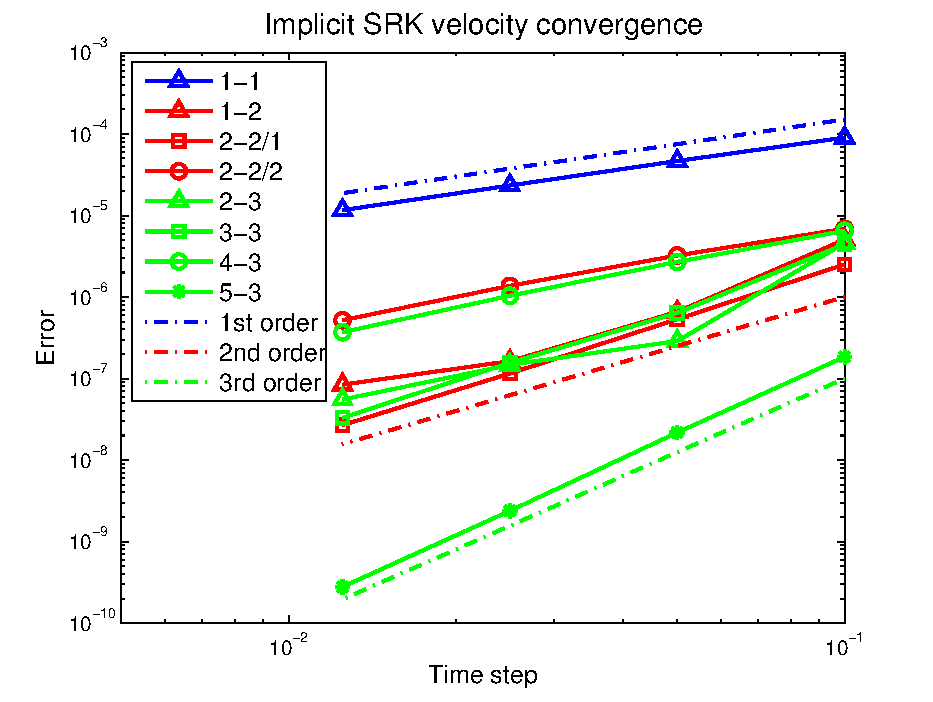
\includegraphics[width=0.49\textwidth]{Figures/Chapter6/analytical/vel_nu1dot0E+00_implconv}}    
  \subfigure[Pressure convergence, $\nu=1.0$]{\label{fig:IMEX_implcnv_RK_pre_analytical_nu1.0}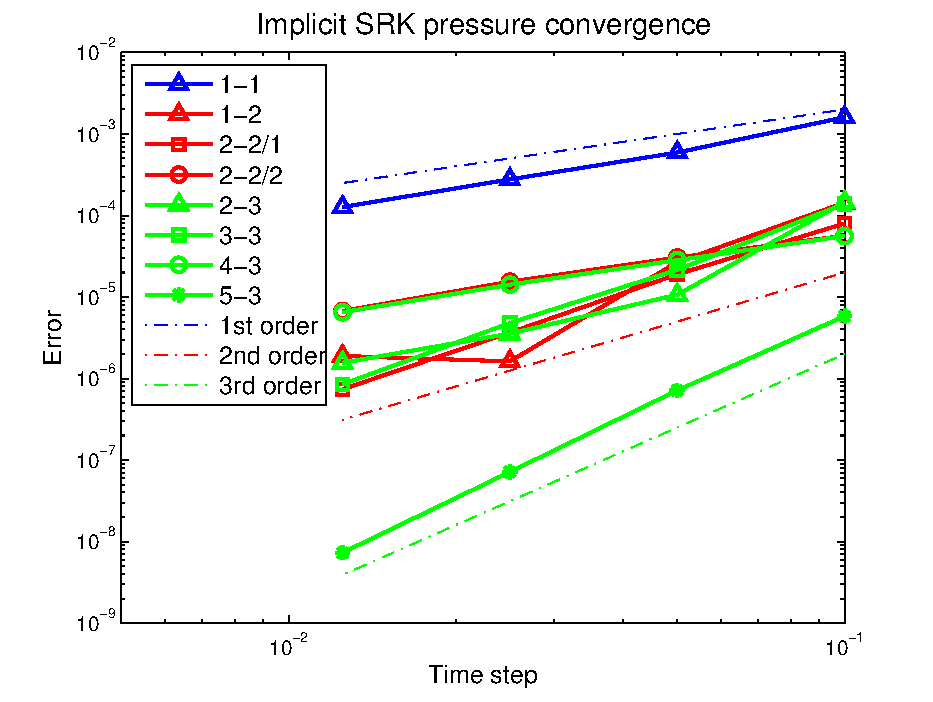
\includegraphics[width=0.49\textwidth]{Figures/Chapter6/analytical/pre_nu1dot0E+00_implconv}}\\
  \subfigure[Velocity convergence, $\nu=0.1$]{\label{fig:IMEX_implcnv_RK_vel_analytical_nu0.1}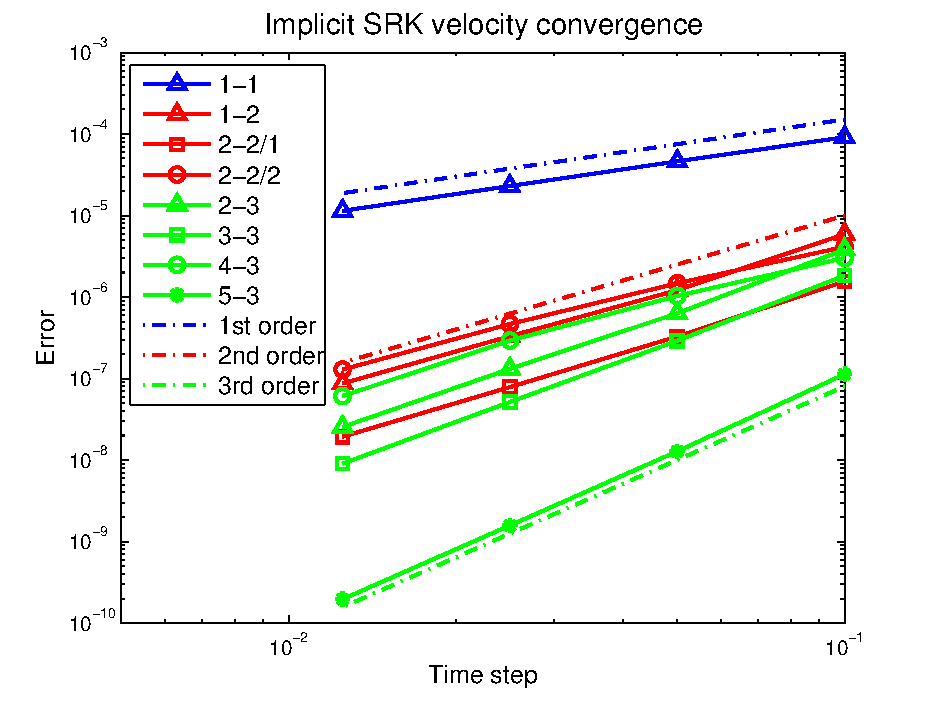
\includegraphics[width=0.49\textwidth]{Figures/Chapter6/analytical/vel_nu1dot0E-01_implconv}}    
  \subfigure[Pressure convergence, $\nu=0.1$]{\label{fig:IMEX_implcnv_RK_pre_analytical_nu0.1}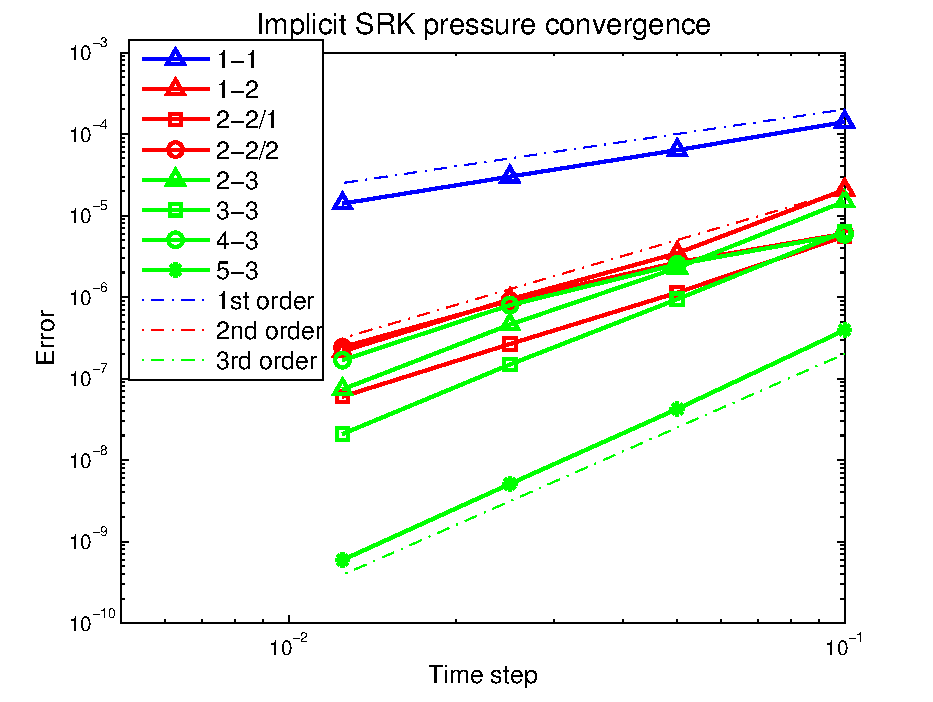
\includegraphics[width=0.49\textwidth]{Figures/Chapter6/analytical/pre_nu1dot0E-01_implconv}}\\
  \subfigure[Velocity convergence, $\nu=0.01$]{\label{fig:IMEX_implcnv_RK_vel_analytical_nu0.01}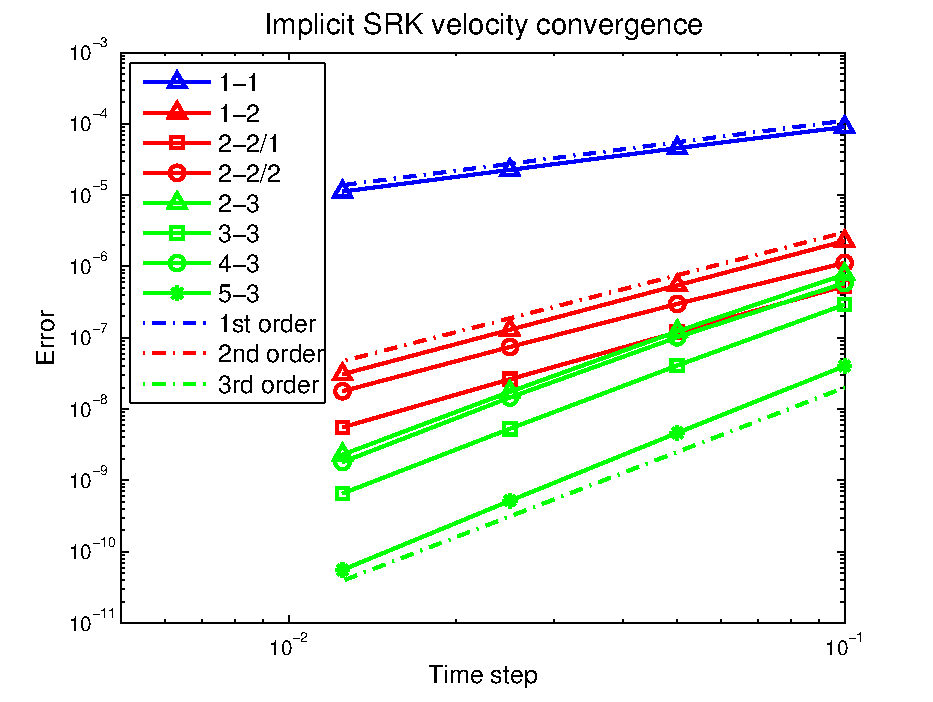
\includegraphics[width=0.49\textwidth]{Figures/Chapter6/analytical/vel_nu1dot0E-02_implconv}}    
  \subfigure[Pressure convergence, $\nu=0.01$]{\label{fig:IMEX_implcnv_RK_pre_analytical_nu0.01}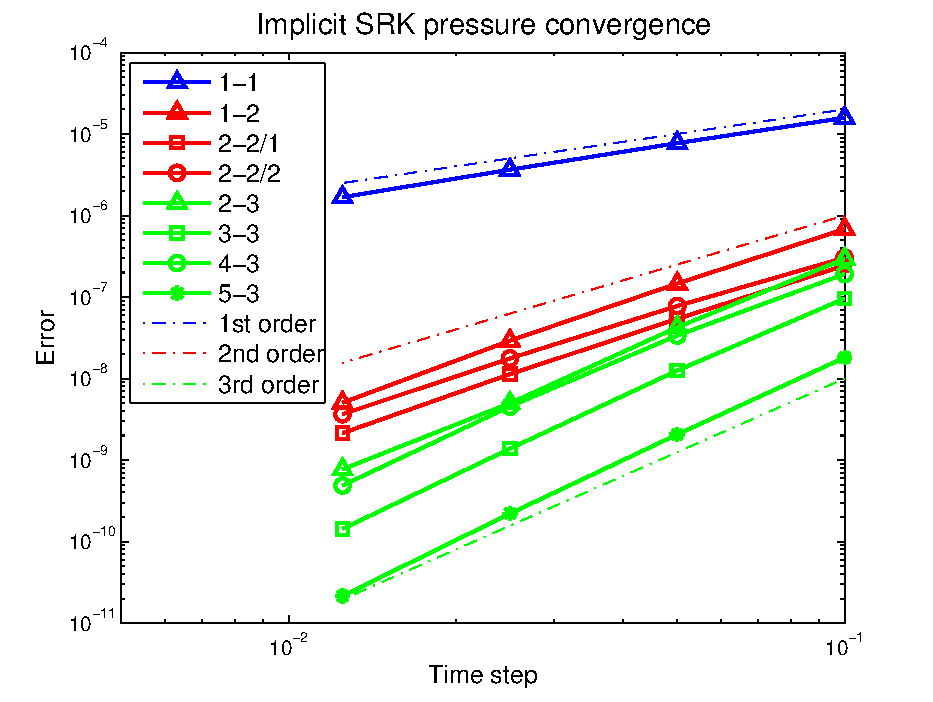
\includegraphics[width=0.49\textwidth]{Figures/Chapter6/analytical/pre_nu1dot0E-02_implconv}}
  \caption{Fully implicit SRK.}
  \label{fig:IMEX_implcnv_RK_analytical}
\end{figure}

\paragraph{IMEX-SRK.}

In this case the SRK scheme is defined only with the diffusive term integrated implicitly, while the convective one is treated explicitly. Then, the operators $\mathcal{F}$ and $\mathcal{G}$ will be
$$\mathcal{F}(\U):=-K\U,\quad\quad\mbox{and}\quad\quad\mathcal{G}(\U,\P):=\F-C(\U)\U-G\P.$$
Note that for this case, there will be the limitation on the hyperbolic ${\rm CFL}_u$ number, which is less restrictive than the parabolic one. As it is seen in Table \ref{tab:CFL}, it is always less than $1.0$ for the chosen time step sizes.

Fig. \ref{fig:IMEX_explcnv_RK_analytical} depicts the velocity and pressure convergence rate using different viscosities for this second case. 
For the highest viscosity $\nu=1.0$ (Figs. \ref{fig:IMEX_explcnv_RK_vel_analytical_nu1.0} and \ref{fig:IMEX_explcnv_RK_pre_analytical_nu1.0}), we note that almost all methods perform in a similar way as the fully implicit SRK case, with the difference that scheme \textit{(3-3)} is also showing an order reduction in its convergence rate, being of 2nd order. In this case, we can state that the \textit{(5-3)} scheme is the only third-order scheme that does not show an order reduction in the time convergence, although for the smallest time steps, the velocity convergence rate is a little bit lower than 3.

When we reduce the viscosity to $\nu=0.1$ or $\nu=0.01$, all schemes show the same behaviour as the fully implicit SRK case, see Figs. \ref{fig:IMEX_explcnv_RK_vel_analytical_nu0.1}, \ref{fig:IMEX_explcnv_RK_pre_analytical_nu0.1},  \ref{fig:IMEX_explcnv_RK_vel_analytical_nu0.01}, and  \ref{fig:IMEX_explcnv_RK_pre_analytical_nu0.01}. 
\begin{figure}[h!]
  \centering
  \subfigure[Velocity convergence, $\nu=1.0$]{\label{fig:IMEX_explcnv_RK_vel_analytical_nu1.0}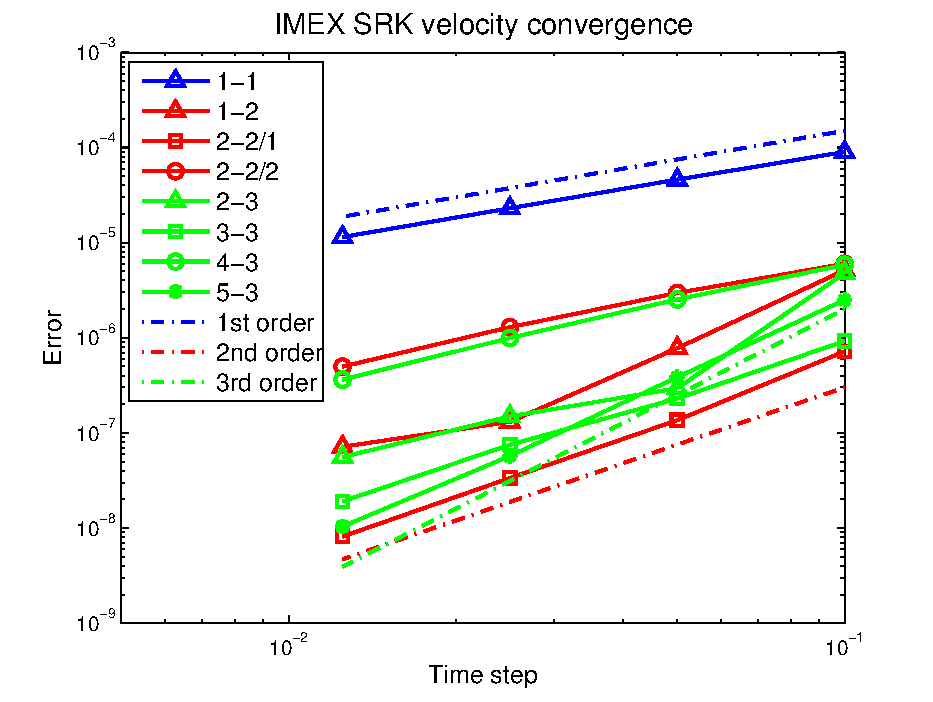
\includegraphics[width=0.49\textwidth]{Figures/Chapter6/analytical/vel_nu1dot0E+00_explconv}}    
  \subfigure[Pressure convergence, $\nu=1.0$]{\label{fig:IMEX_explcnv_RK_pre_analytical_nu1.0}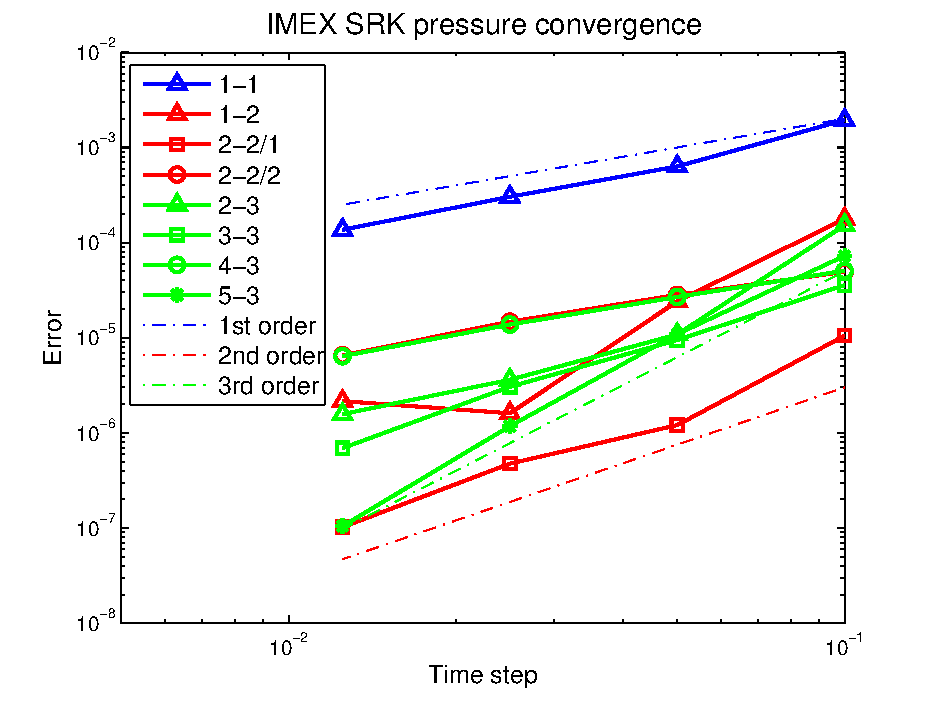
\includegraphics[width=0.49\textwidth]{Figures/Chapter6/analytical/pre_nu1dot0E+00_explconv}}\\
  \subfigure[Velocity convergence, $\nu=0.1$]{\label{fig:IMEX_explcnv_RK_vel_analytical_nu0.1}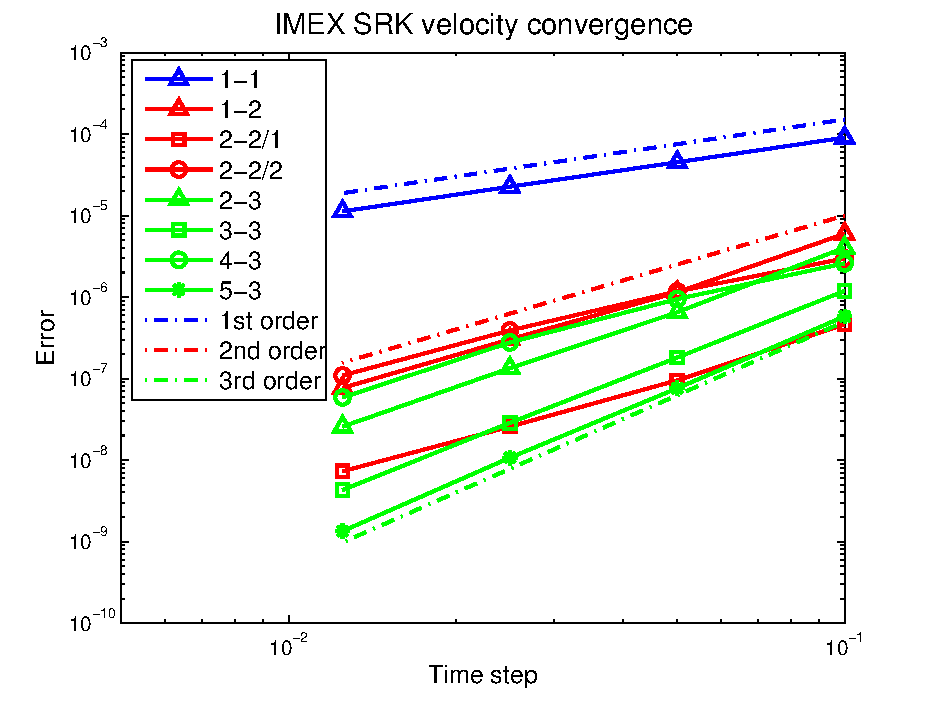
\includegraphics[width=0.49\textwidth]{Figures/Chapter6/analytical/vel_nu1dot0E-01_explconv}}    
  \subfigure[Pressure convergence, $\nu=0.1$]{\label{fig:IMEX_explcnv_RK_pre_analytical_nu0.1}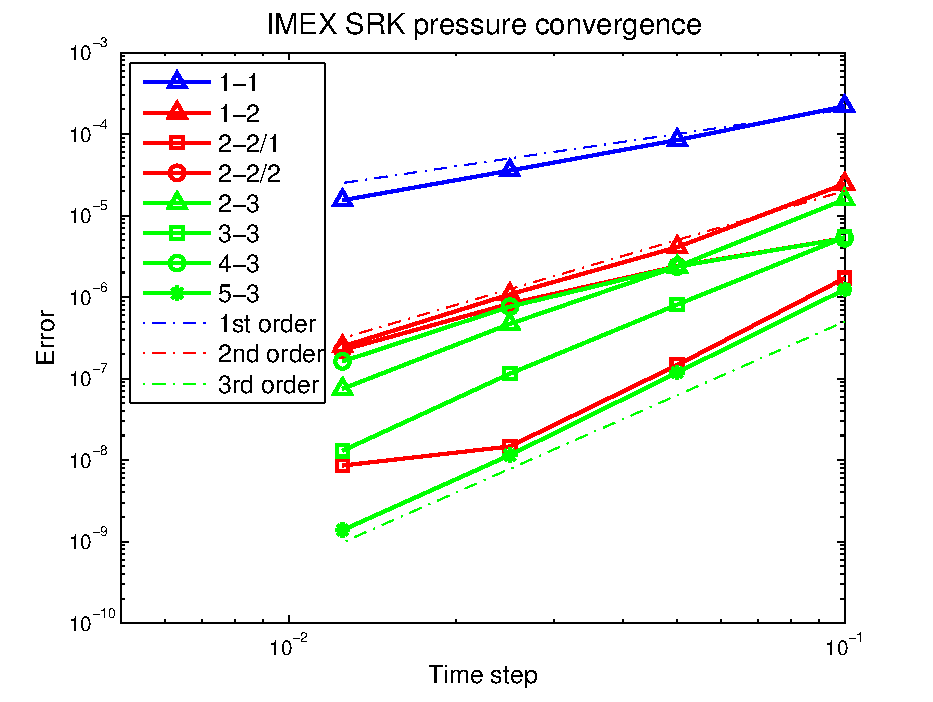
\includegraphics[width=0.49\textwidth]{Figures/Chapter6/analytical/pre_nu1dot0E-01_explconv}}\\
  \subfigure[Velocity convergence, $\nu=0.01$]{\label{fig:IMEX_explcnv_RK_vel_analytical_nu0.01}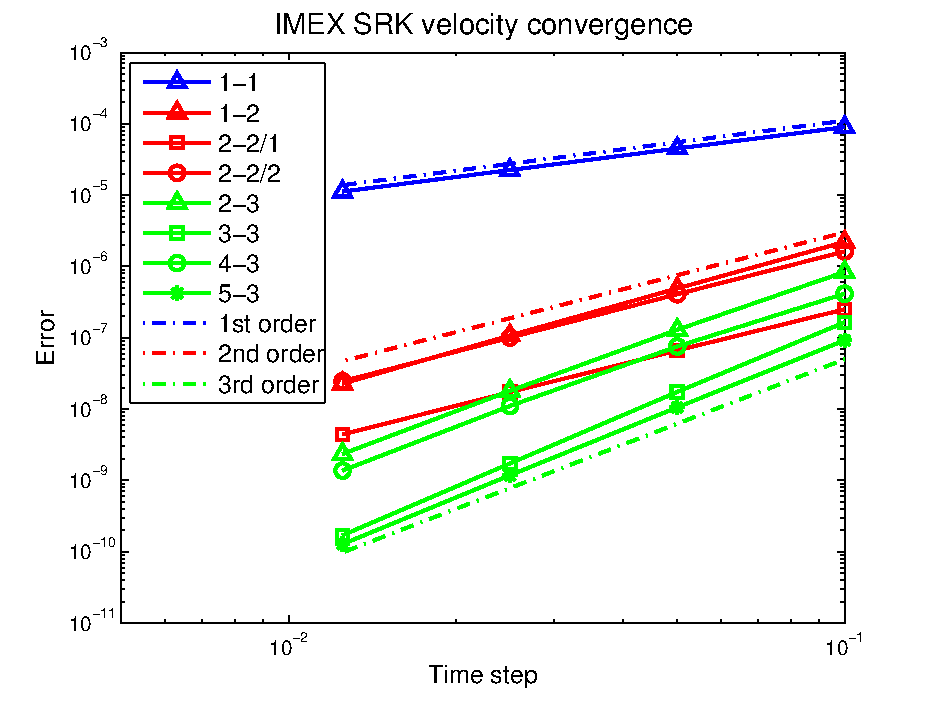
\includegraphics[width=0.49\textwidth]{Figures/Chapter6/analytical/vel_nu1dot0E-02_explconv}}    
  \subfigure[Pressure convergence, $\nu=0.01$]{\label{fig:IMEX_explcnv_RK_pre_analytical_nu0.01}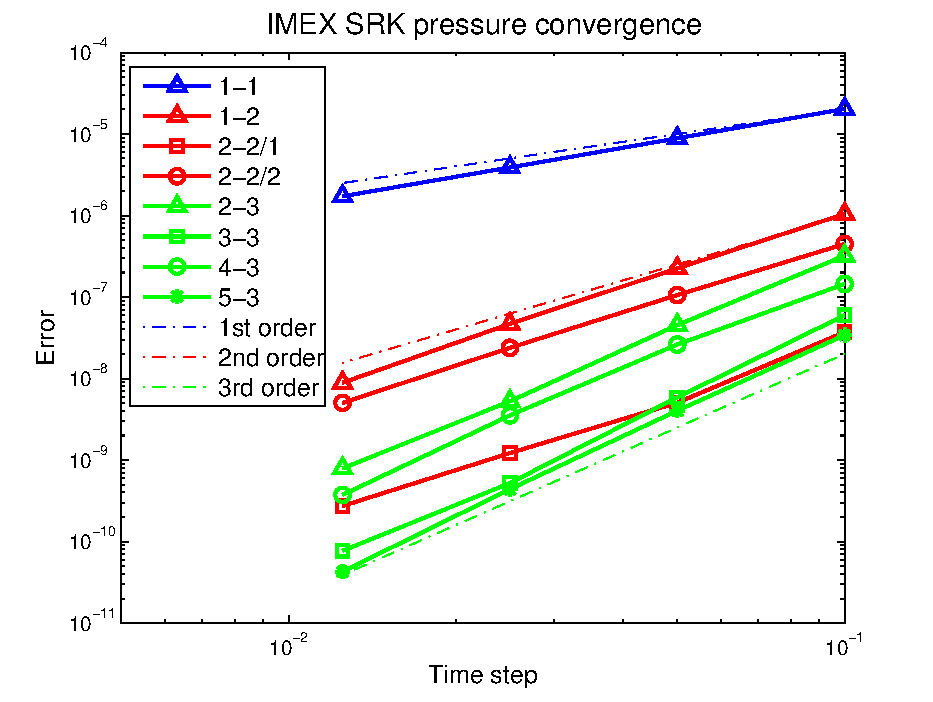
\includegraphics[width=0.49\textwidth]{Figures/Chapter6/analytical/pre_nu1dot0E-02_explconv}}
  \caption{SRK convergence with convection integrated explicitly and diffusion integrated implicitly.}
  \label{fig:IMEX_explcnv_RK_analytical}
\end{figure}
Let us note that the \textit{(2-2/1)} scheme has much lower error in the IMEX-SRK case than in the fully implicit SRK case.

\paragraph{Fully explicit SRK.}

Finally we test the fully explicit situation, which consist on sending all terms to the right-hand side of the equation. The operators $\mathcal{F}$ and $\mathcal{G}$ in  Eqs. (\ref{eq-C6_IMEX_NS_up}) and \Eq{C6_IMEX_NS_up_n+1} will read
$$\mathcal{F}(\U):=0,\quad\quad\mbox{and}\quad\quad\mathcal{G}(\U,\P):=\F-(\K+\C(\U))\U-G\P.$$
In this case the {CFL} number that limits the stability of the method is given by the parabolic one (${\rm CFL}_\nu$). This is far more restrictive than ${\rm CFL}_u$ in the IMEX case, and for the setting described above we get unstable results. Only when the viscosity is $\nu=0.01$, the ${\rm CFL}_\nu$ values are in the order or smaller than the critical value $1.0$.

Fig. \ref{fig:Expl_RK_analytical} depicts the convergence rate for this case, where we see that for the velocity (Fig. \ref{fig:Expl_RK_vel_analytical_nu0.01}) and the pressure (Fig. \ref{fig:Expl_RK_pre_analytical_nu0.01}) fields the order of convergence is the desired one for most of the schemes, except for the \textit{(5-3)} scheme which converges with a higher order. Here does not appear the order reduction phenomena since it is not present for explicit schemes.
\begin{figure}[h!]
  \centering
  \subfigure[Velocity convergence, $\nu=0.01$]{\label{fig:Expl_RK_vel_analytical_nu0.01}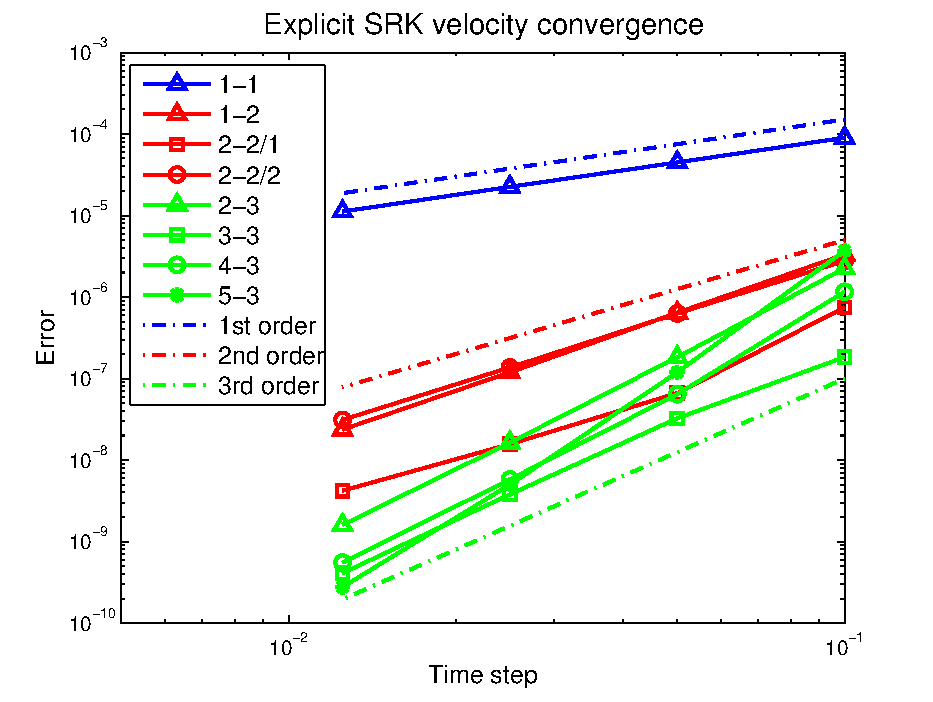
\includegraphics[width=0.49\textwidth]{Figures/Chapter6/analytical/vel_nu1dot0E-02_explfull}}    
  \subfigure[Pressure convergence, $\nu=0.01$]{\label{fig:Expl_RK_pre_analytical_nu0.01}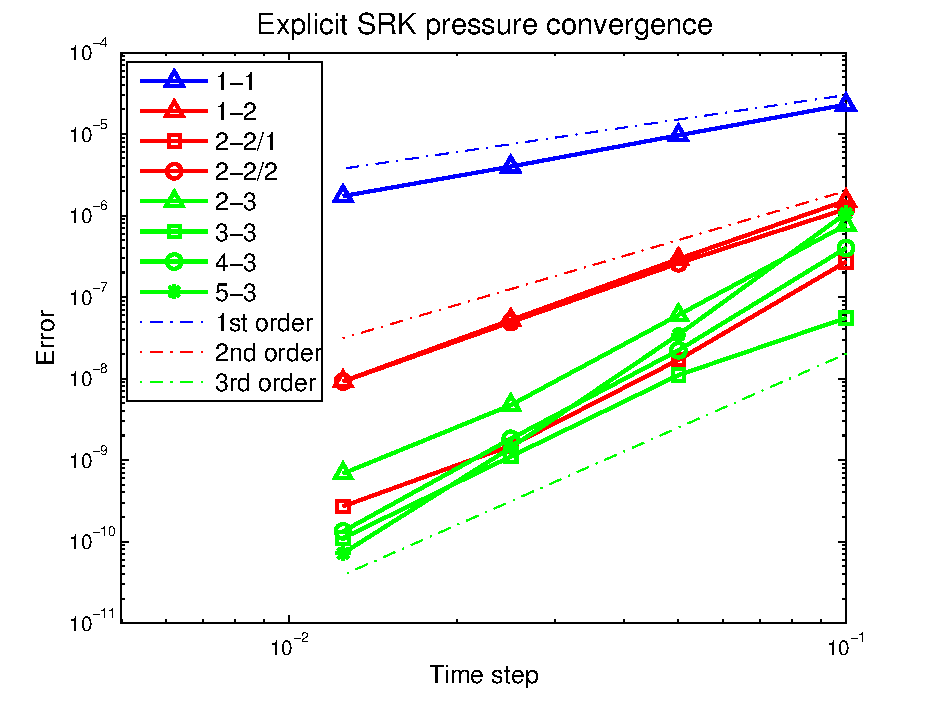
\includegraphics[width=0.49\textwidth]{Figures/Chapter6/analytical/pre_nu1dot0E-02_explfull}}
  \caption{Fully explicit SRK convergence.}
  \label{fig:Expl_RK_analytical}
\end{figure}


\paragraph{Discrete divergence constraint preservation.}

As stated in Proposition \ref{prop2}, the discrete divergence constraint is preserved when the strongly imposed Dirichlet data is a polynomial of order at most $p-1$ in time. In order to show this phenomena we solve the same problem given by \Eq{C6_analytical_u}-\Eq{C6_analytical_p}, but considering a second order polynomial for the time dependency. The analytical solution to be solved in this case will be
\begin{align*}
%\label{eq-C6_analytical_u_t2}
&\u(x,y,t) = \left( \begin{tabular}{l}
$x$\\
$-y$
\end{tabular}\right)t^2,\\
%\label{eq-C6_analytical_p_t2}
&p(x,y) = x+y.
\end{align*}
This problem is solved with the fully implicit SRK method from $t=0$ to {$t=2.0$} using a time step size { $\delta t=1.0\cdot10^{-2}$} and a viscosity $\nu=0.01$. { The linear solver tolerance has been set equal to $1.0\cdot10^{-8}$, and for the implicit version, the nonlinear tolerance is $1.0\cdot10^{-6}$}. In Fig. \ref{fig:RK_analytical_t2} the evolution of $\|\nabla \cdot \u\|$ is depicted for all schemes considered in \ref{appendix:Butcher_tab}, for both the implicit and explicit versions of the SRK method. We see that for the first-order \textit{(1-1)} scheme the discrete divergence constraint is not preserved as it was expected. Moreover, the second-order schemes seem to give really accurate results when evaluating the discrete divergence, even when the time dependence of the solution is of order 2. { The \textit{(2-2/2)} and \textit{(4-3)} schemes, which do not satisfy the condition $b_i=\hat{b_i}$ for $i=1,...,s$, have the worst performance compared to the other methods of the same order. Although the errors are very small, we can observe the effect of the accumulation of solver error commented in Remark \ref{remark3}, which leads to an increasing value of $\|\nabla \cdot \u\|$. In any case, the third order schemes that have been proved to preserve the discrete divergence constraint (see Proposition \ref{prop2}) keep $\|\nabla \cdot \u\|$ below $10^{-9}$.
}
\begin{figure}[h!]
  \centering
  \subfigure[Implicit SRK]{\label{fig:Impl_RK_analytical_t2}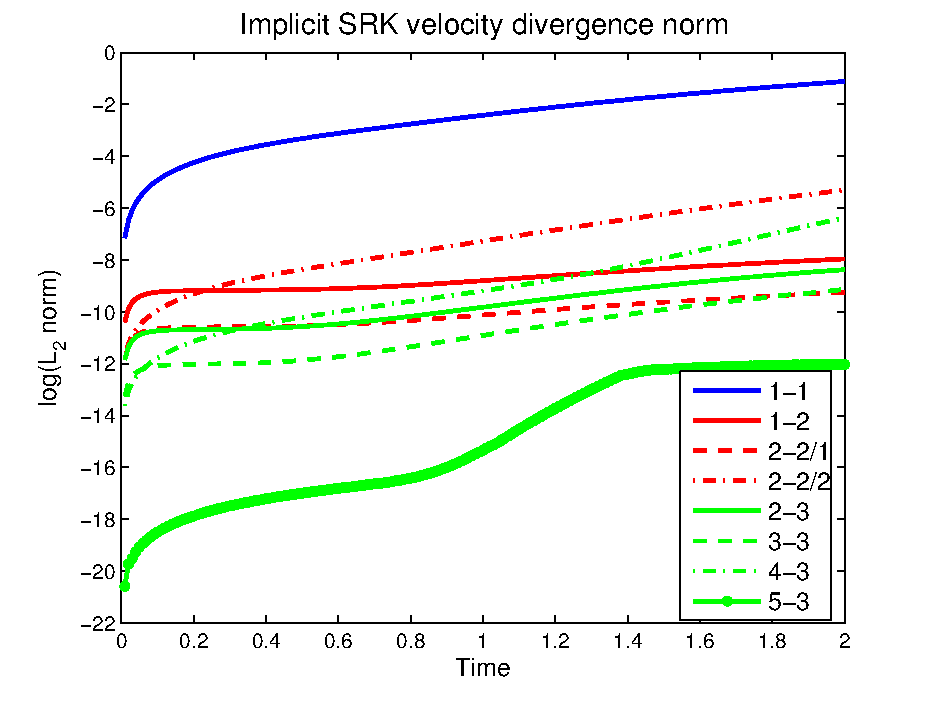
\includegraphics[width=0.49\textwidth]{Figures/Chapter6/analytical/div_norm_implconv_0_2_dt0dot1e-01}}    
  \subfigure[Explicit SRK]{\label{fig:Expl_RK_analytical_t2}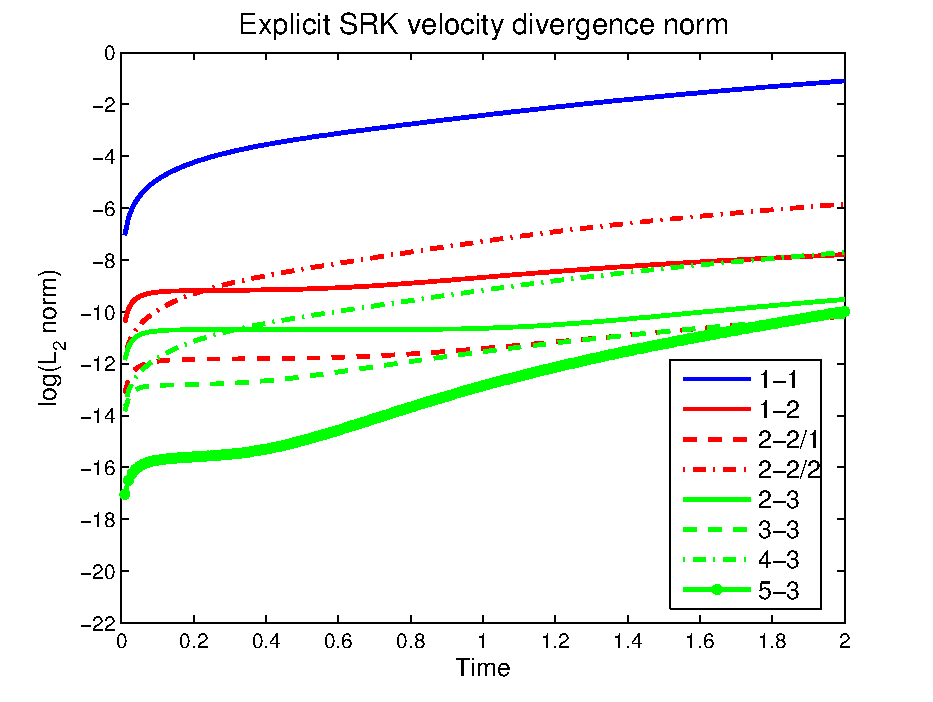
\includegraphics[width=0.49\textwidth]{Figures/Chapter6/analytical/div_norm_explconv_0_2_dt0dot1e-01}}
  \caption{ $\| \nabla \cdot \u\|$ for the implicit and explicit SRK schemes.}
  \label{fig:RK_analytical_t2}
\end{figure}
%\begin{figure}[h!]
%  \centering
%  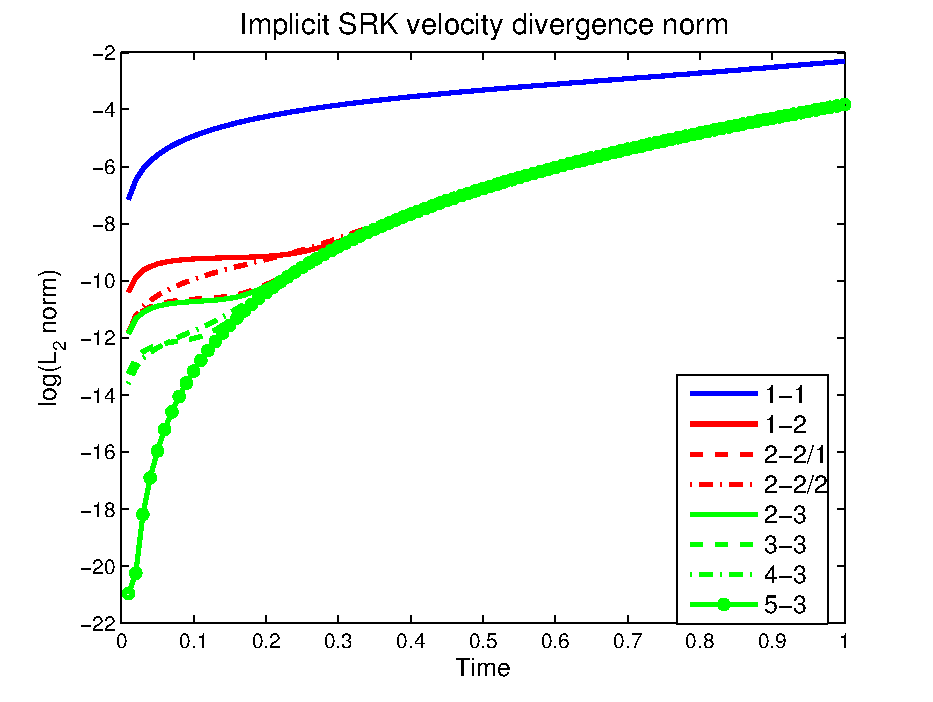
\includegraphics[width=0.49\textwidth]{Figures/analytical/div_norm_implconv_0_1_dt0dot1e-01}
%  %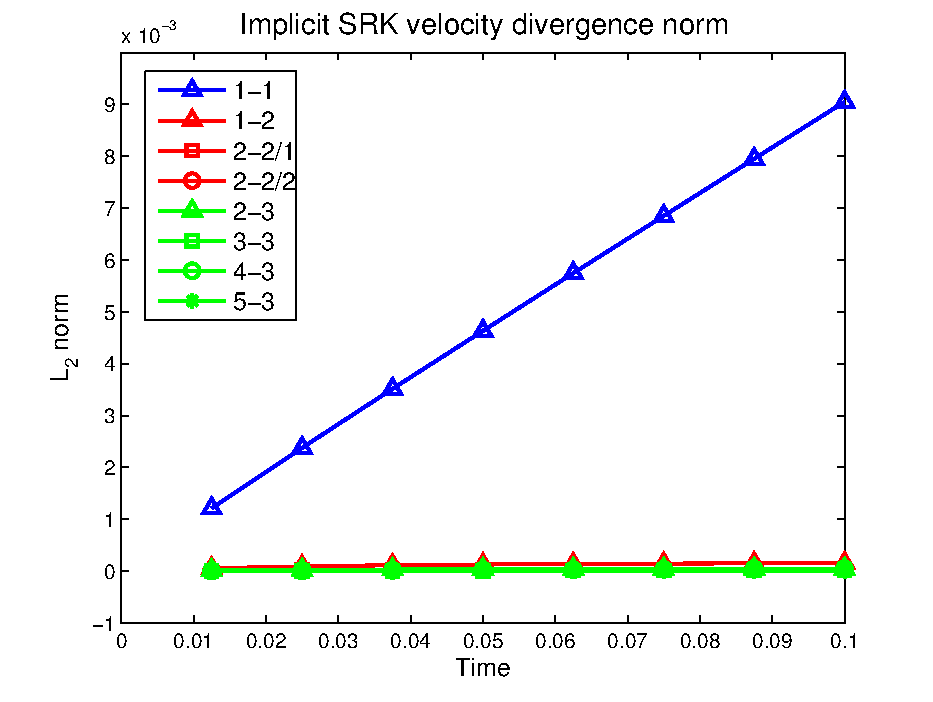
\includegraphics[width=0.49\textwidth]{Figures/analytical/div_nu1dot0E-02_implconv_t2}  
%  \caption{Residual of the divergence constraint equation for the fully explicit SRK scheme.}
%  \label{fig:Impl_RK_analytical_t2}
%\end{figure}

\subsection{Beltrami flow}
In the manufactured analytical solution stated in \Eq{C6_analytical_u}-\Eq{C6_analytical_p} the spatial error is not present since the solution belongs to the FE space. In order to check the behaviour of SRK methods when solving problems with spatial error originated by the discretization in space, we consider an analytical solution that does not belong to the FE space. A 3D Beltrami flow like the one defined in \cite{ethier_exact_1994} is used in this subsection, but in this case a pressure with no dependence in time is defined. The flow is solved in a cube centered on $(x,y,z)=(0,0,0)$ and with a edge size $L=2$, the viscosity of the problem in this case is set as $\nu=0.01$.
\begin{align}
\label{eq-C6_beltrami_u}
&\u(x,y,z,t) = \left( \begin{tabular}{l}
$-a\left[e^{ax}\sin(ay+dz)+e^{az}\cos(ax+dy)\right]$\\
$-a\left[e^{ay}\sin(az+dx)+e^{ax}\cos(ay+dz)\right]$\\
$-a\left[e^{az}\sin(ax+dy)+e^{ay}\cos(az+dx)\right]$
\end{tabular}\right)e^{-d^2t},\\
\label{eq-C6_beltrami_p}
&p(x,y,z) = -\frac{a^2}{2}\left[e^{2ax}+e^{2ay}+e^{2ay}+2\sin(ax+dy)\cos(az+dx)e^{a(y+z)}\right. \\\nonumber
&\left.+2\sin(ay+dz)\cos(ax+dy)e^{a(z+x)}+2\sin(az+dx)\cos(ay+dz)e^{a(x+y)}\right].
\end{align}
To analyze the effect of the spatial error we solve the problem with the analytical solution \Eq{C6_beltrami_u}-\Eq{C6_beltrami_p} refining both in time and space keeping the ratio $\delta t/h$ constant. The problem is solved using $Q_2/Q_1$ elements with the IMEX SRK method, for all schemes stated in \ref{appendix:Butcher_tab}. A first result is obtained setting the $\delta t/h=0.01$, with the time step sizes $\delta t=\{5.0\cdot10^{-3},2.5\cdot10^{-3},1.25\cdot10^{-3},6.25\cdot10^{-4}\}$ and solving from $t=0$ till $T=5.0\cdot10^{-3}$. A second test is done with a smaller ratio, $\delta t/h=0.002$, being the time steps sizes $\delta t=\{1.0\cdot10^{-3},5.0\cdot10^{-4},2.5\cdot10^{-4},1.25\cdot10^{-4}\}$ from $t=0$ till $T=1.0\cdot10^{-3}$.
\begin{figure}[h!]
  \centering
  \subfigure[Error convergence, $\frac{\delta t}{h}=0.01$]{\label{fig:beltrami_0.01}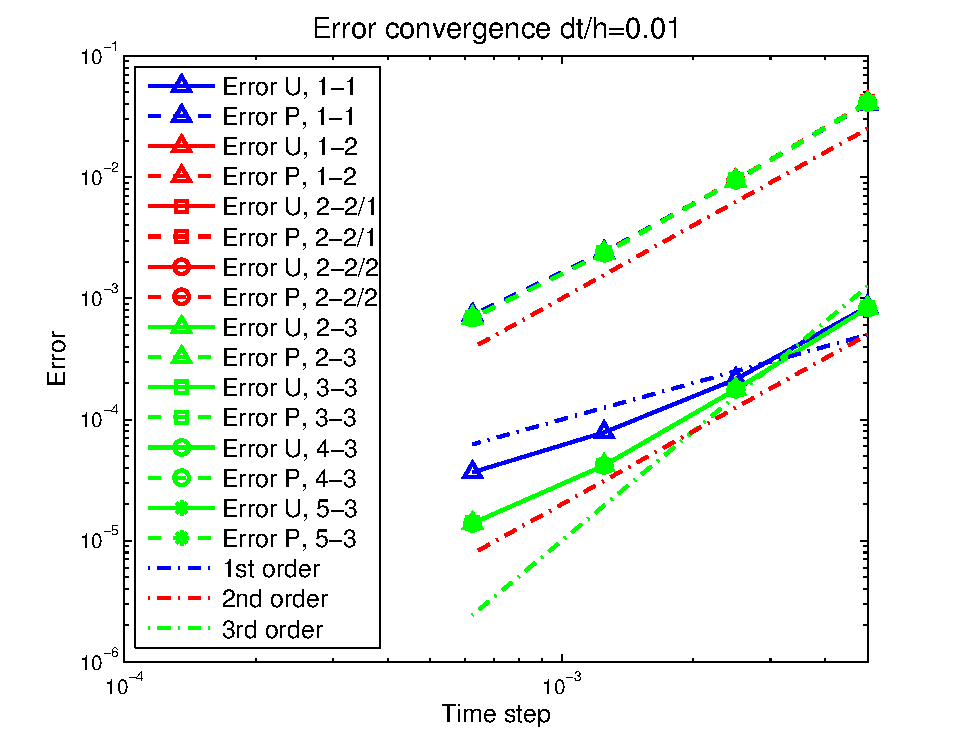
\includegraphics[width=0.49\textwidth]{Figures/Chapter6/analytical/dth_01}}    
  \subfigure[Error convergence, $\frac{\delta t}{h}=0.002$]{\label{fig:beltrami_0.002}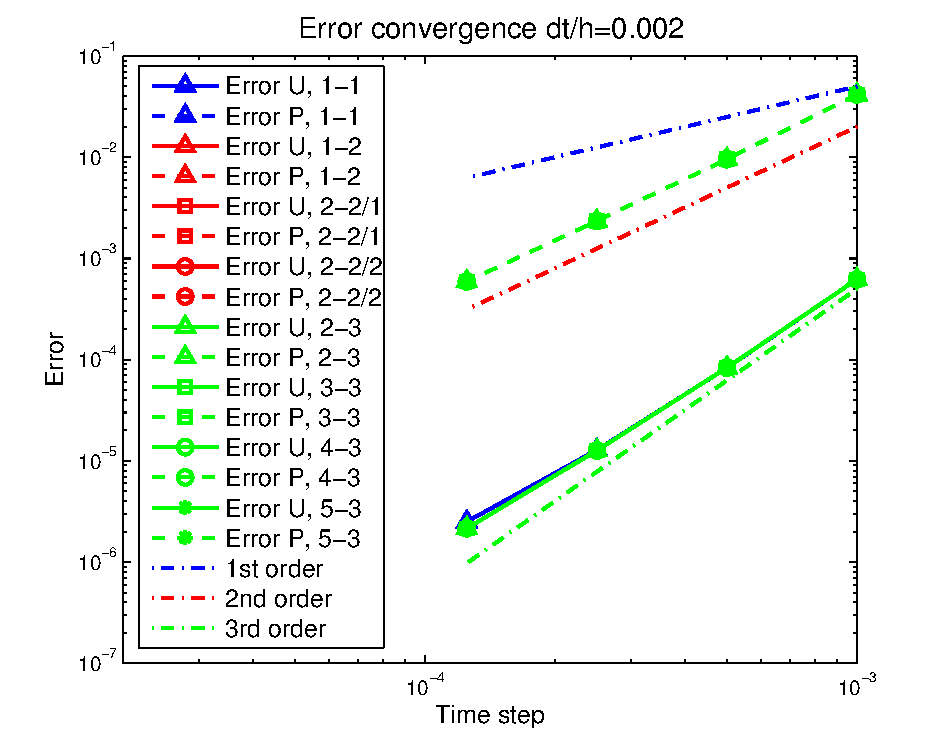
\includegraphics[width=0.49\textwidth]{Figures/Chapter6/analytical/dth_002}}
  \caption{Beltrami flow error convergence (red and blue lines below green line).}
  \label{fig:beltrami}
\end{figure}
In Fig. \ref{fig:beltrami} the error convergence for both velocity and pressure fields is depicted. The results for the case with $\frac{\delta t}{h}=0.01$ are shown in Fig. \ref{fig:beltrami_0.01}, where we clearly see that the convergence rate for the pressure field is two, the one prescribed by the spatial discretization error, so here all schemes give the same result since the spatial error prevails over the temporal error. But looking at the velocity field results at the same figure, it is seen that the third-order of convergence given by the theoretical spatial error convergence is reduced. Here we see how the first order scheme \textit{(1-1)} starts loosing the convergence rate given by the spatial error and exhibits the convergence rate prescribed by the temporal discretization. All the other schemes converge with a second order slope, even the third-order schemes. This order reduction phenomena is also observed in \cite{sanz-serna_convergence_1986} when both $\delta t$ and $h$ are refined simultaneously.
When we select a smaller ratio of $\delta t/h$, see Fig. \ref{fig:beltrami_0.002}, the temporal error is masked by the spatial error, giving a third-order convergence for the velocity field and a second-order convergence for the pressure field. A little reduction of the order is observed at the smallest time step sizes for the velocity field in Fig. \ref{fig:beltrami_0.002}.

\subsection{2D Laminar flow around a cylinder}
\label{subsec-C6_cylinder}
Once studied the behaviour of the different methods proposed in Section \ref{sec-C6_SRK_developement} for a manufactured analytical solution, we study a widely used laminar flow benchmark which is the flow around a cylinder for a low Reynolds number $Re=100$. A detailed overview of benchmark computations of laminar flow around a cylinder are given in \cite{schafer_benchmark_1996}. The test performed in the current work is called \textit{2D-2} in that paper and is defined as shown in Fig. \ref{fig:Cyl_geom}. It basically consists in a rectangular channel with a cylinder located near the inflow boundary. A non-slip condition is imposed in the cylinder wall and the channel walls that are perpendicular to the flow direction ($x$).
\begin{figure}[h!]
  \centering
  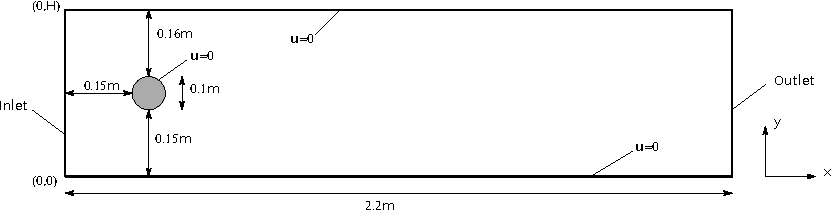
\includegraphics[width=\textwidth]{Figures/Chapter6/geom_2D} 
  \caption{Flow around a cylinder test geometry.}
  \label{fig:Cyl_geom}
\end{figure}
The inflow condition is
$$\u(0,y,t)=\left(\begin{array}{c}
u_x\\
u_y\\
\end{array}\right)=\left(\begin{array}{c}
4U_m\frac{y(H-y)}{H^2}\\
0\\
\end{array}\right),$$
with the maximum velocity $U_m=1.5$ m/s and $H=0.41$ the channel height.

Our aim is not only to see the order of convergence of the time integration schemes proposed, but also to compare the results with a detailed benchmark that has been used to test different algorithmic approaches. Then, we compute the parameters needed for this comparison, namely the drag coefficient $c_D$, the lift coefficient $c_L$, and the pressure difference $\Delta P$ as functions of time for one period $[t_0,t_0+1/f]$, $f$ being the frequency of separation. The values that we will use in the comparison are the maximum drag coefficient $c_{D_{\rm max}}$, the maximum lift coefficient $c_{L_{\rm max}}$ , the Strouhal number ${\rm St}$ and the pressure difference $\Delta P(t)$ at $t=t_0+0.5/f$. The initial time $t_0$ should correspond to the flow state with $c_{L_{\rm max}}$. The drag coefficient $c_D$ and  the lift coefficient $c_L$ are given by $$c_D=\frac{2F_D}{\rho\bar{U}^2D},\quad\quad c_L=\frac{2F_L}{\rho\bar{U}^2D},$$
being $\rho=1.0$ the fluid density, $D=0.1$ the cylinder diameter, and $\bar{U}=1.0$ the mean velocity. The drag $F_D$ and lift $F_L$ forces are defined as $$F_D=\int_S\left(\rho\nu\frac{\partial v_t}{\partial n}n_y-pn_x\right){\rm d}S,\quad\quad F_L=-\int_S\left(\rho\nu\frac{\partial v_t}{\partial n}n_x-pn_y\right){\rm d}S,$$
with $S$ the cylinder surface and $n$ the normal vector on $S$, with $n_x$ and $n_y$ the $x$-component and $y$-component, respectively. $v_t$ is the tangential velocity on $S$ for the tangent vector $t=(n_y,-n_x)$. These surface integrals are computed as the residual of the weak form on boundary nodes, as advocated in \cite{brezzi_variational_2001} for accuracy reasons.

In order to reduce computational cost, we first compute the flow from $t=0$ to $t=8.0$ with a monolithic fully implicit Crank-Nicolson scheme with a time step equal to $\delta t=0.05$. In Fig. \ref{fig:Cyl_vorti} we show the vorticity field at $t=8.0$. It can be seen that at that time the flow is fully developed. So, at $t=8.0$ we can start the computations with the different schemes studied in this work. The computations are performed from $t=8.0$ to $t=8.4$, ensuring that we have two maximums of the lift coefficient, so we have a complete period of data after the first lift coefficient maximum. 

\begin{figure}[h!]
  \centering
  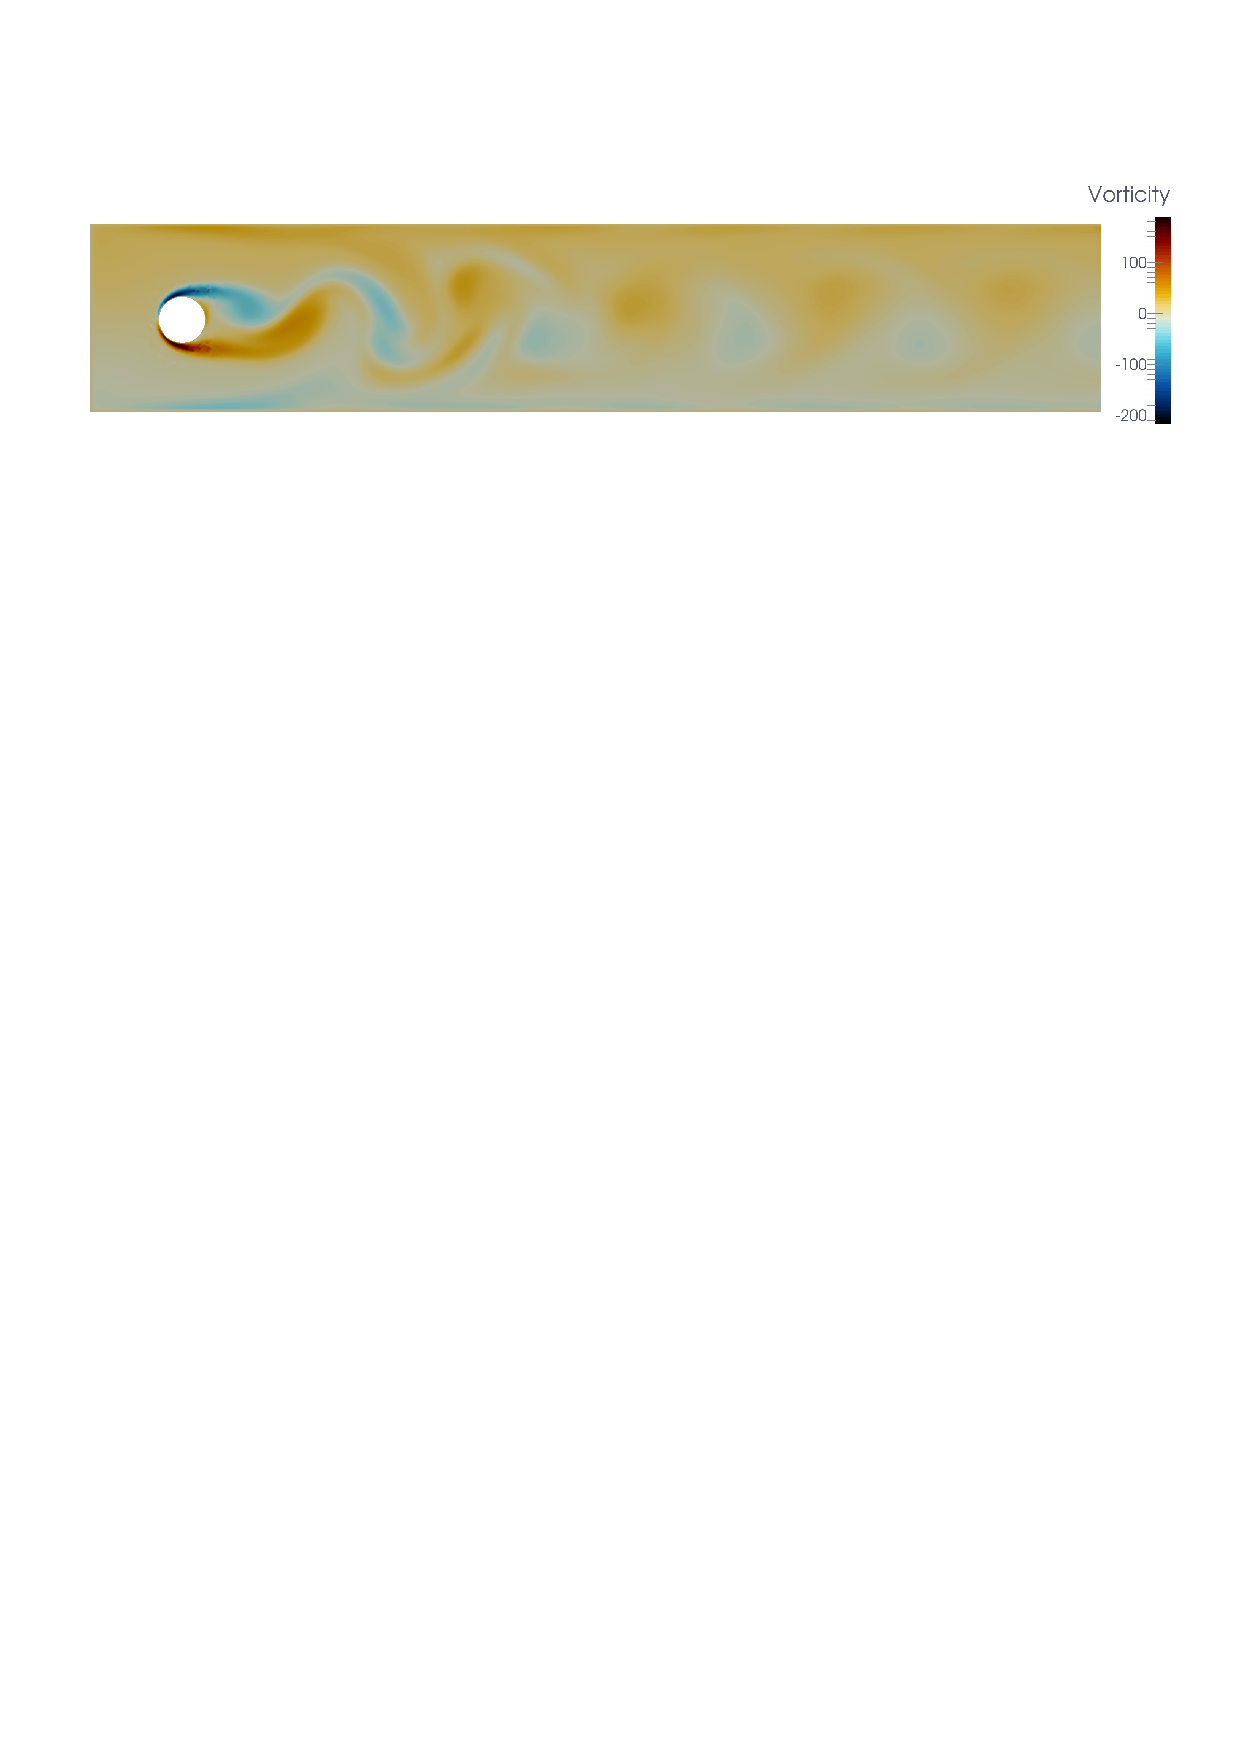
\includegraphics[clip=true,trim=1.5cm 22.5cm 1cm 3cm,width=\textwidth]{Figures/Chapter6/cylinder/vorticity}
  \caption{Vorticity field at $t=8.0$.}
  \label{fig:Cyl_vorti}
\end{figure}

As exposed in the discussion of results in \cite{schafer_benchmark_1996}, the use of explicit schemes for the time integration of laminar flows is not an efficient approach. The restriction on the time step size to ensure stability of the method is critical since the physical time scale may be much larger. %However, in this subsection we will focus on the performance in terms of convergence, not in efficiency with respect to the fully implicit method. In Subsection \ref{subsec-C6_TGV} the efficiency of IMEX schemes is assessed for a turbulent test, where the physical time scale is not so large and may be smaller than the critical one. 
As a result, we will only focus on the fully implicit and IMEX approaches. In this test we consider two different situations: 1) Fully implicit SRK scheme; 2) SRK scheme with diffusive term integrated implicitly and convective term explicitly.

This test is solved using a mesh with 13886 $Q_2/Q_1$ elements, for all the schemes defined by the Butcher tableaus exposed in \ref{appendix:Butcher_tab} and for several time step sizes. In particular, the problem is solved with $\delta t=\{2.0\cdot10^{-2},1.0\cdot10^{-2},5.0\cdot10^{-3},2.5\cdot10^{-3},1.25\cdot10^{-3}\}$ for each scheme. Furthermore, an extra computation for the \textit{(3-3)} scheme is done with $\delta t=3.125\cdot10^{-4}$ in order to have a more accurate result from which we can compare to do the convergence analysis.

In \cite{schafer_benchmark_1996} there is not a prescribed correct value for the benchmark quantities, but there is a range within which most of the reported values are located. Then, we expect that our computation results will fit into these bounds.

\paragraph{Fully implicit SRK.}

Here, as the flow is laminar, we do not expect the nonlinearity of the convective term to play a decisive role in the computational cost. So, it seems natural to consider an implicit treatment of this term, especially taking into account that the explicit treatment of this term involves time stepping restrictions. Thus, the schemes used in this first case are given by defining the operators $\mathcal{F}$ and $\mathcal{G}$ in Eqs. (\ref{eq-C6_IMEX_NS_up}) and \Eq{C6_IMEX_NS_up_n+1} as
$$\mathcal{F}(\U):=\F-(\K+\C(\U))\U,\quad\quad\mbox{and}\quad\quad\mathcal{G}(\U,\P):=-G\P.$$

Let us point out that for this test the \textit{(1-2)} and \textit{(2-3)} schemes are unstable for the largest time step sizes, {i.e.} $\delta t\geq 1.25\cdot10^{-3}$ for the \textit{(1-2)} scheme and $\delta t\geq2.5\cdot10^{-3}$ for the \textit{(2-3)} scheme. Therefore, these two schemes will not be taken into account in the results shown in this first case. The benchmark quantities of the different computations are given in Table \ref{tab:IMEX-RK_cyl2d_implconv}, together with the lower and upper bounds of the results in \cite{schafer_benchmark_1996}. It is seen that most of the computed quantities fit into the benchmark bounds; the Strouhal number seems to be a little bit greater than the upper bound in some cases. Note that aside the Strouhal number, the other quantities converge to a value that is inside the benchmark range. As it is expected, the schemes with higher order have more results in the correct range and give very accurate results earlier when we refine the time step.

\begin{table}[h!]
	\caption{Benchmark 2D-2 results with implicit convection.}
	\label{tab:IMEX-RK_cyl2d_implconv}
	\centering
	\begin{tabular} {cccccc}
		\toprule
			Scheme & $\delta t$ & $c_{D_{max}}$ & $c_{L_{max}}$ & $St$ & $\Delta P$  \\
		\midrule
		\midrule
			$(1-1)$ & 2.000e-02 & 3.1984 & 0.8261 & 0.2941 & 2.4291 \\ 
			$(1-1)$ & 1.000e-02 & 3.2024 & 0.8704 & 0.2941 & 2.4398 \\ 
			$(1-1)$ & 5.000e-03 & 3.2108 & 0.9158 & 0.3030 & 2.4568 \\ 
			$(1-1)$ & 2.500e-03 & 3.2182 & 0.9441 & 0.3030 & 2.4700 \\ 
			$(1-1)$ & 1.250e-03 & 3.2230 & 0.9598 & 0.3042 & 2.4780 \\  
		\midrule
			$(2-2/1)$ & 2.000e-02 & 3.2423 & 1.0121 & 0.3125 & 2.5082 \\ 
			$(2-2/1)$ & 1.000e-02 & 3.2329 & 1.0039 & 0.3030 & 2.4867 \\ 
			$(2-2/1)$ & 5.000e-03 & 3.2304 & 1.0008 & 0.3077 & 2.4852 \\ 
			$(2-2/1)$ & 2.500e-03 & 3.2298 & 1.0009 & 0.3053 & 2.4884 \\ 
			$(2-2/1)$ & 1.250e-03 & 3.2296 & 1.0007 & 0.3065 & 2.4883 \\  
		\midrule
			$(2-2/2)$ & 2.000e-02 & 3.2418 & 1.0819 & 0.3125 & 2.4954 \\ 
			$(2-2/2)$ & 1.000e-02 & 3.2323 & 1.0063 & 0.3030 & 2.4835 \\ 
			$(2-2/2)$ & 5.000e-03 & 3.2301 & 0.9973 & 0.3077 & 2.4845 \\ 
			$(2-2/2)$ & 2.500e-03 & 3.2297 & 0.9997 & 0.3053 & 2.4883 \\ 
			$(2-2/2)$ & 1.250e-03 & 3.2296 & 1.0003 & 0.3065 & 2.4883 \\  
		\midrule
			$(3-3)$ & 2.000e-02 & 3.2361 & 1.0138 & 0.3125 & 2.5027 \\ 
			$(3-3)$ & 1.000e-02 & 3.2304 & 1.0013 & 0.3030 & 2.4849 \\ 
			$(3-3)$ & 5.000e-03 & 3.2298 & 0.9999 & 0.3077 & 2.4848 \\ 
			$(3-3)$ & 2.500e-03 & 3.2296 & 1.0007 & 0.3053 & 2.4883 \\ 
			$(3-3)$ & 1.250e-03 & 3.2296 & 1.0006 & 0.3065 & 2.4883 \\  
		\midrule
			$(4-3)$ & 2.000e-02 & 3.2321 & 1.1003 & 0.3125 & 2.4788 \\ 
			$(4-3)$ & 1.000e-02 & 3.2285 & 0.9948 & 0.3030 & 2.4802 \\ 
			$(4-3)$ & 5.000e-03 & 3.2285 & 0.9954 & 0.3077 & 2.4839 \\ 
			$(4-3)$ & 2.500e-03 & 3.2294 & 1.0000 & 0.3053 & 2.4881 \\ 
			$(4-3)$ & 1.250e-03 & 3.2296 & 1.0005 & 0.3065 & 2.4882 \\ 
		\midrule
			$(5-3)$ & 2.000e-02 & 3.2249 & 0.9770 & 0.3125 & 2.4951 \\ 
			$(5-3)$ & 1.000e-02 & 3.2290 & 0.9977 & 0.3030 & 2.4843 \\ 
			$(5-3)$ & 5.000e-03 & 3.2295 & 0.9995 & 0.3077 & 2.4847 \\ 
			$(5-3)$ & 2.500e-03 & 3.2296 & 1.0006 & 0.3053 & 2.4883 \\ 
			$(5-3)$ & 1.250e-03 & 3.2296 & 1.0006 & 0.3065 & 2.4883 \\ 
		\midrule
		\midrule
			\multicolumn{2}{c}{lower bound} & 3.2200 & 0.9900 & 0.2950 & 2.4600 \\
			\multicolumn{2}{c}{upper bound} & 3.2400 & 1.0100 & 0.3050 & 2.5000 \\
		\bottomrule
	\end{tabular}
\end{table}

To check the convergence in time of the different time integration schemes, we perform a convergence analysis computing the $\ell^\infty$-norm of the velocity and the pressure errors, $e_u$ and $e_p$. In this case, the solution is not compared against an analytical one but computed with a finer time step ($\delta t=3.125\cdot10^{-4}$) with the \textit{(3-3)} scheme. The reason of this choice is related to the efficiency of this scheme, discussed below.

In Fig. \ref{fig:IMEX_RK_cyl_conv} we show the convergence rate for both velocity and pressure fields, Figs. \ref{fig:IMEX_RK_vel_cyl_implconv} and  \ref{fig:IMEX_RK_pre_cyl_implconv}, respectively. A first conclusion that we can make is that for the largest time steps the order of convergence is not the prescribed one, especially for the first order scheme. It is explained by the fact that the largest time step sizes are greater than the one required for stability purposes when a fully-explicit scheme is used. %,%the largest time step size, $\delta t=2.0\cdot10^{-2}$, provides very inaccurate results, even though the computations do not blow up for this time step size. It is explained by the fact that this time step size is about two orders of magnitude the explicit one, required for stability purposes. 
%It seems that there is a kind of {CFL} condition on the velocity-pressure splitting approach that makes the computed results wrong for time steps larger than a certain time step size. It is important to highlight that this {CFL} condition is about one order of magnitude greater than the ${\rm CFL}_u$ and ${\rm CFL}_\nu$ ones. 
%In the following case, with the convection integrated explicitly, we will discuss this issue with more detail. 
 For the time steps smaller than $2.0\cdot10^{-2}$ the convergence rates are the expected ones, with the exception of \textit{(1-1)} and \textit{(4-3)} schemes, with a convergence rate lower than the expected one.
\begin{figure}[h!]
  \centering
  \subfigure[Velocity convergence]{\label{fig:IMEX_RK_vel_cyl_implconv}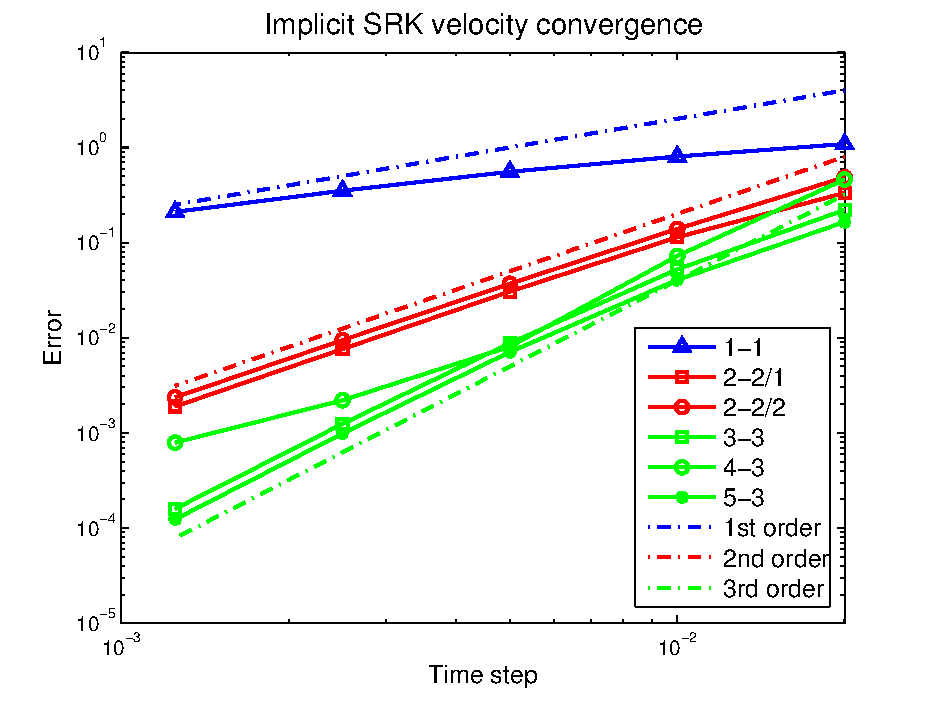
\includegraphics[width=0.49\textwidth]{Figures/Chapter6/cylinder/vel_implconv}}    
  \subfigure[Pressure convergence]{\label{fig:IMEX_RK_pre_cyl_implconv}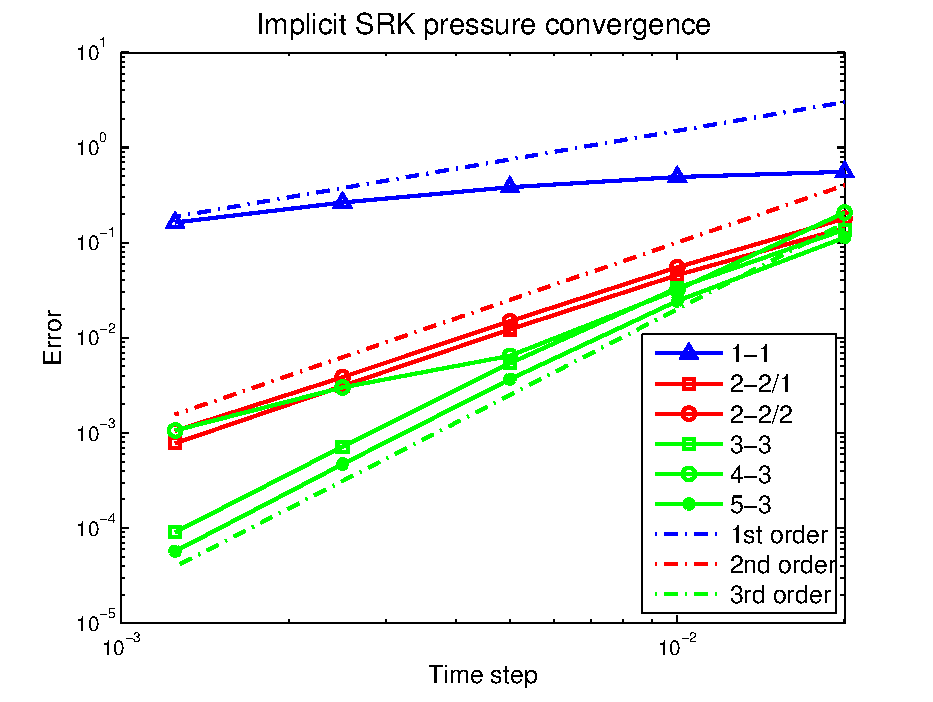
\includegraphics[width=0.49\textwidth]{Figures/Chapter6/cylinder/pre_implconv}}
  \caption{Fully implicit SRK convergence.}
  \label{fig:IMEX_RK_cyl_conv}
\end{figure}
%Going back to Fig. \ref{fig:IMEX_RK_pre_cyl_implconv}, one may realize that the last points of the \textit{(3-3)} and \textit{(5-3)} schemes do not follow the correct convergence rate line. This behaviour is due to the nonlinear tolerance of the problem solution, which is set equal to $10^{-4}$. The accumulation of the error given by this weak nonlinear tolerance among the time steps results in a solution that does not follow the expected convergence rate.

Fig. \ref{fig:IMEX_RK_cyl_conv} shows that the most accurate schemes are \textit{(3-3)} and \textit{(5-3)}. Now, let us analyze the computational cost of these methods based on the CPU time for a given target error. %\comment{All this section must be re-written without that point now.}
\begin{figure}[h!]
  \centering
  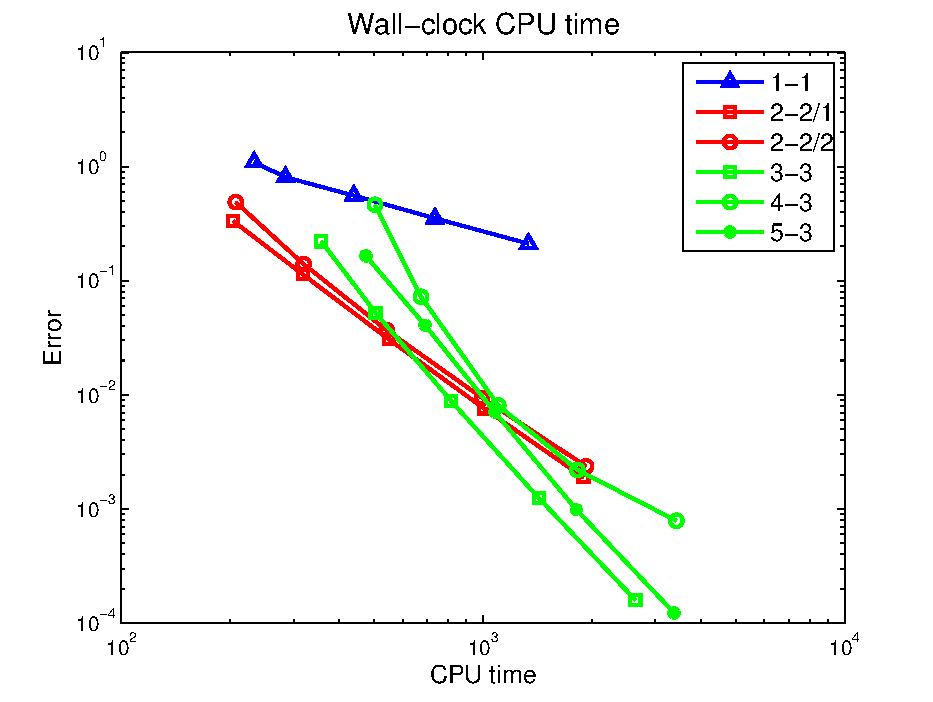
\includegraphics[width=0.49\textwidth]{Figures/Chapter6/cylinder/Efficiency}  
  \caption{Fully implicit SRK CPU time efficiency.}
  \label{fig:IMEX_RK_cyl_effi}
\end{figure}
In Fig. \ref{fig:IMEX_RK_cyl_effi} it is clearly seen that the most efficient scheme is \textit{(3-3)}, even for relatively high error ($\sim4\cdot10^{-2}$). For larger target errors, the \textit{(2-2/1)} schemes is competitive. We note that the first order \textit{(1-1)} scheme is not competitive at all, since the error is too large and there is no significant gain in CPU time. %Thus, as the most efficient is the \textit{(3-3)} scheme, the computation with a finer time step to compare the solution is done with this scheme.

\paragraph{IMEX-SRK.}

In this case, we consider an explicit time integration approach of the convective term. That is to define the operators $\mathcal{F}$ and $\mathcal{G}$ in  Eqs. (\ref{eq-C6_IMEX_NS_up}) and \Eq{C6_IMEX_NS_up_n+1} as
$$\mathcal{F}(\U):=\F-K\U,\quad\quad\mbox{and}\quad\quad\mathcal{G}(\U,\P):=C(\U)-G\P.$$

As it has been exposed above, the explicit treatment of the convective term implies time stepping restrictions that are given by the condition on the hyperbolic ${\rm CFL}_u$ number. As the mesh is not homogeneous and the velocity is not the same over all the domain, we can obtain a bound for the maximum ${\rm CFL}_u$ number taking the maximum value over all the elements. %velocity and the minimum element size, $u_{\rm max}=2.23$ and $h_{min}=0.0024$.
 With these parameters, the maximum ${\rm CFL}_u$ depending on the time step size will be of the order shown in Table \ref{tab:CFLu_cyl}.

\begin{table}[h]
\caption{${\rm CFL}_u$ values.}
\label{tab:CFLu_cyl}
\centering
\begin{tabular}{cc}
\toprule
$\delta t$&${\rm CFL}_u$\\
\midrule
\midrule
$2.0\cdot10^{-2}$&$6.81$\\
$1.0\cdot10^{-2}$&$3.48$\\
$5.0\cdot10^{-3}$&$1.79$\\
$2.5\cdot10^{-3}$&$0.91$\\
$1.25\cdot10^{-3}$&$0.46$\\
$6.25\cdot10^{-4}$&$0.21$\\
$3.125\cdot10^{-4}$&$0.11$\\
$1.5625\cdot10^{-4}$&$0.05$\\
$7.8125\cdot10^{-5}$&$0.03$\\
\bottomrule
\end{tabular}
\end{table}

Looking at Table \ref{tab:CFLu_cyl} we see that in this case the time step needs to be much smaller than in the previous case if we want to guarantee a stable solution. For the implicit treatment of the convective term, for time step sizes below or equal to  $\delta t\leq 1.0\cdot10^{-2}$, the method is stable and gives good convergence rates. Here, for this time step we see that we have a ${\rm CFL}_u\sim3.4$, which is grater than the critical $\sim1.0$. %\comment{Then, we can state that the {CFL} condition given by the velocity-pressure segregation is about one order of magnitude higher than the hyperbolic ${\rm CFL}_u$ for this particular test.}

In effect, the largest time step size for which all the schemes give stable results for this case is $\delta t=3.125\cdot10^{-4}$. Some schemes also are stable for $\delta t=6.25\cdot10^{-4}$ or even for $\delta t=1.25\cdot10^{-3}$, but no one is stable for $\delta t=2.5\cdot10^{-3}$, which is of the order of the critical time step size. Thus, it is clear that for this type of problems, an explicit time integration of the convective term implies the use of much smaller time steps than for an implicit time integration of this term.

In Table \ref{tab:IMEX-RK_cyl2d_explconv} we show the benchmark quantities of the cases that attained convergence, till $\delta t=1.5625\cdot10^{-4}$. It is clearly seen that for such small time step sizes all the results are very similar, showing that the IMEX-SRK scheme also gives good results considering the explicit integration of the convective term, whenever the time step is sufficiently small to give a stable result. The results that are out of the range are in italics.
\begin{table}[h!]
	\caption{Benchmark 2D-2 results with explicit convection.}
	\label{tab:IMEX-RK_cyl2d_explconv}
	\centering
	\begin{tabular} {cccccc}
		\toprule
			Scheme & $\delta t$ & $c_{D_{max}}$ & $c_{L_{max}}$ & $St$ & $\Delta P$  \\
		\midrule
		\midrule
			$(1-1)$ & 3.125e-04 & 3.2272 & \textit{0.9882} & \textit{0.3059} & 2.4862 \\ 
			$(1-1)$ & 1.563e-04 & 3.2280 & 0.9944 & \textit{0.3062} & 2.4879 \\ 
		\midrule
			$(1-2)$ & 3.125e-04 & 3.2296 & 1.0006 & \textit{0.3068} & 2.4891 \\ 
			$(1-2)$ & 1.563e-04 & 3.2296 & 1.0006 & \textit{0.3065} & 2.4893 \\ 
		\midrule
			$(2-2/1)$ & 6.250e-04 & 3.2296 & 1.0006 & \textit{0.3065} & 2.4891 \\ 
			$(2-2/1)$ & 3.125e-04 & 3.2296 & 1.0006 & \textit{0.3065} & 2.4895 \\ 
			$(2-2/1)$ & 1.563e-04 & 3.2296 & 1.0006 & \textit{0.3065} & 2.4893 \\ 
		\midrule
			$(2-2/2)$ & 6.250e-04 & 3.2296 & 1.0006 & \textit{0.3065} & 2.4892 \\ 
			$(2-2/2)$ & 3.125e-04 & 3.2296 & 1.0006 & \textit{0.3065} & 2.4896 \\ 
			$(2-2/2)$ & 1.563e-04 & 3.2296 & 1.0006 & \textit{0.3065} & 2.4893 \\ 
		\midrule
			$(2-3)$ & 3.125e-04 & 3.2296 & 1.0006 & \textit{0.3065} & 2.4895 \\ 
			$(2-3)$ & 1.563e-04 & 3.2296 & 1.0006 & \textit{0.3065} & 2.4893 \\ 
		\midrule
			$(3-3)$ & 6.250e-04 & 3.2296 & 1.0006 & \textit{0.3065} & 2.4891 \\ 
			$(3-3)$ & 3.125e-04 & 3.2296 & 1.0006 & \textit{0.3065} & 2.4895 \\ 
			$(3-3)$ & 1.563e-04 & 3.2296 & 1.0006 & \textit{0.3065} & 2.4893 \\ 
		\midrule
			$(4-3)$ & 6.250e-04 & 3.2296 & 1.0006 & \textit{0.3065} & 2.4891 \\ 
			$(4-3)$ & 3.125e-04 & 3.2296 & 1.0006 & \textit{0.3065} & 2.4895 \\ 
			$(4-3)$ & 1.563e-04 & 3.2296 & 1.0006 & \textit{0.3065} & 2.4893 \\ 
		\midrule
			$(5-3)$ & 6.250e-04 & 3.2296 & 1.0006 & \textit{0.3065} & 2.4891 \\ 
			$(5-3)$ & 3.125e-04 & 3.2296 & 1.0006 & \textit{0.3065} & 2.4895 \\ 
			$(5-3)$ & 1.563e-04 & 3.2296 & 1.0006 & \textit{0.3065} & 2.4893 \\ 
		\midrule
		\midrule
			\multicolumn{2}{c}{lower bound} & 3.2200 & 0.9900 & 0.2950 & 2.4600 \\
			\multicolumn{2}{c}{upper bound} & 3.2400 & 1.0100 & 0.3050 & 2.5000 \\
		\bottomrule
	\end{tabular}
\end{table}

%Concerning about the convergence in time, Fig. \ref{fig:IMEX_RK_cyl_conv_explcnv} depicts the convergence rate of all the schemes. Here, we show the $L^\infty$-norm of the error, $e_u$ and $e_p$, comparing each solution against the same reference solution used in the implicit convection integration case.
%
%\begin{figure}[h!]
%  \centering
%  \subfigure[Velocity convergence]{\label{fig:IMEX_RK_vel_cyl_explconv}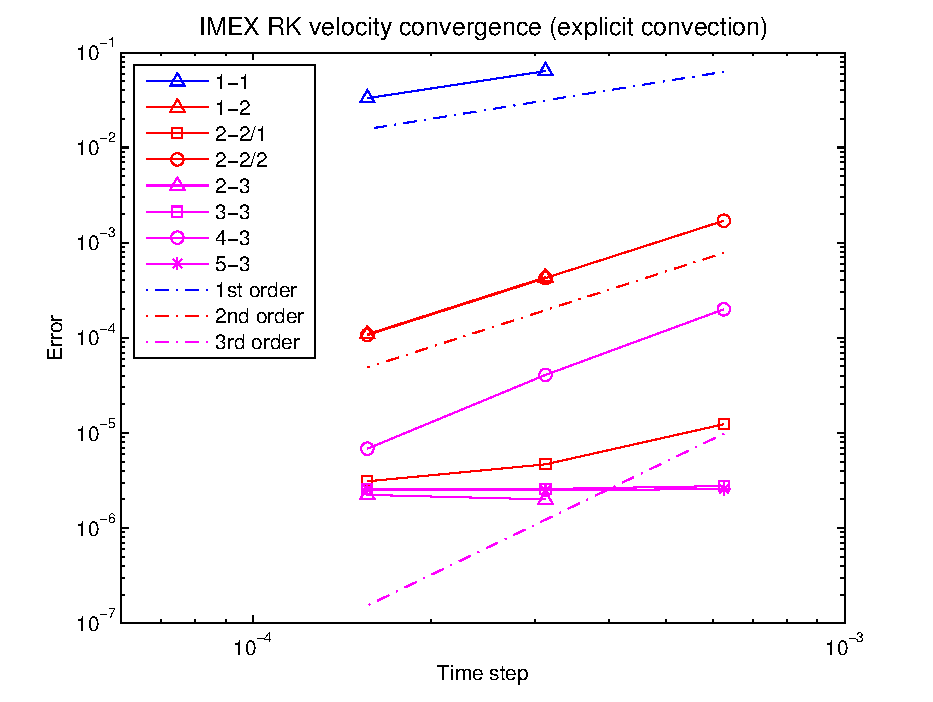
\includegraphics[width=0.49\textwidth]{Figures/cylinder/vel_explconv}}    
%  \subfigure[Pressure convergence]{\label{fig:IMEX_RK_pre_cyl_explconv}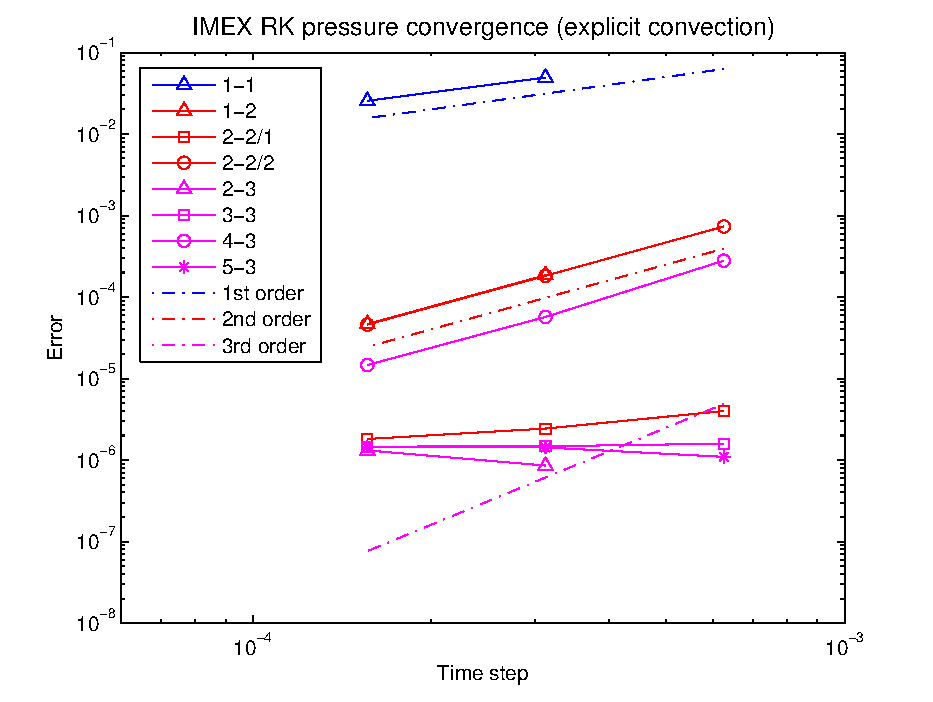
\includegraphics[width=0.49\textwidth]{Figures/cylinder/pre_explconv}}
%  \caption{IMEX-RK convergence with diffusion integrated implicitly and convection explicitly.}
%  \label{fig:IMEX_RK_cyl_conv_explcnv}
%\end{figure}
%Looking at Fig. \ref{fig:IMEX_RK_cyl_conv_explcnv}, we can only extract conclusions for the \textit{(1-1), (1-2), (2-2/2)} and \textit{(4-3)} schemes, since  we obtain a flat convergence rate for the others. This behaviour is caused by the stacking of the solver error, as for these small time steps the number of system resolutions from $t=8.0$ to $t=8.4$ is of the order of $\sim10^4$ and the solver tolerance of the order of $\sim10^{-10}$; it is also affected by the fac that the \emph{exact} solution has been obtained with a time step size similar to the ones considered in this test case (with an implicit method). The expected convergence rate is achieved by \textit{(1-1)}, \textit{(1-2)} and \textit{(2-2/2)} schemes, but not for \textit{(4-3)} scheme which, like the implicit convection version, shows a convergence rate lower than the expected one for either velocity field (Fig. \ref{fig:IMEX_RK_vel_cyl_explconv}) or pressure field (Fig. \ref{fig:IMEX_RK_pre_cyl_explconv}).

%Concerning about the convergence in time, it can be shown that all schemes converge with the same rate as the fully implicit version. As the stable time steps for the explicit convection term integration are so small, it does not make sense to show the convergence rate of the solution error computed between $t=8.0$ and $t=8.4$, since we would see a flat convergence rate stuck at $e_u,e_p\sim10^{-6}$. This behaviour is caused by the stacking of the solver error, as for these small time steps the number of system resolutions from $t=8.0$ to $t=8.4$ is of the order of $\sim10^4$ and the solver tolerance of the order of $\sim10^{-10}$; it is also affected by the fact that the \emph{exact} solution has been obtained with a time step size similar to the ones considered in this test case (with an implicit method).

%\paragraph{Implicit vs. explicit.}

In order to compare the efficiency between the implicit and explicit approaches for the time integration of the convective term for this particular test, we perform the convergence analysis for both methods at $t=8.01$ s. We restrict this test only to the most efficient schemes for each order of approximation, which are \textit{(1-1), (2-2/1)}, and \textit{(3-3)} schemes. %, see Fig. \ref{fig:IMEX_RK_cyl_effi}. 
The results of the convergence in time for this comparison are shown in Fig. \ref{fig:IMEX_RK_cyl_conv_impl_expl}. Unstable results for the explicit convective term integration are not plotted in this figure.

The fully implicit versions of the SRK schemes considered here show a good agreement with the prescribed convergence rate. Furthermore, when the time step is sufficiently small, the explicit version seems to give more accurate results. This is especially remarkable for the \textit{(2-2/1)} scheme, where the differences are bigger. Same conclusions can be pointed out for both velocity and pressure fields, since there are not significant differences between their convergence rates, see Figs. \ref{fig:IMEX_RK_vel_cyl_impl_expl} and  \ref{fig:IMEX_RK_pre_cyl_impl_expl}. 
\begin{figure}[h!]
  \centering
  \subfigure[Velocity convergence]{\label{fig:IMEX_RK_vel_cyl_impl_expl}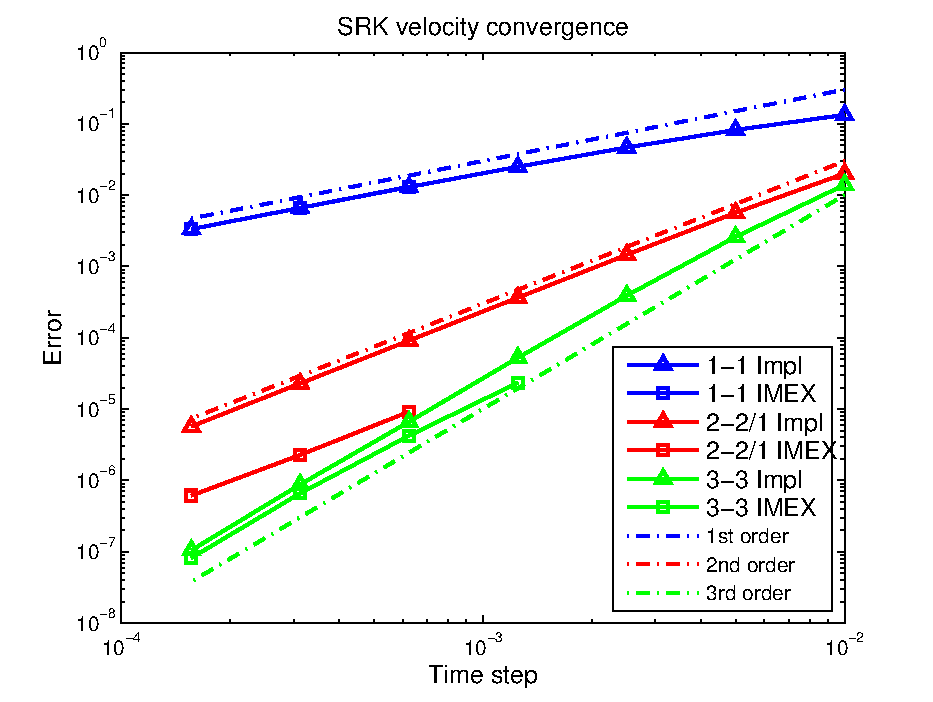
\includegraphics[width=0.49\textwidth]{Figures/Chapter6/cylinder/vel_impl_expl}}    
  \subfigure[Pressure convergence]{\label{fig:IMEX_RK_pre_cyl_impl_expl}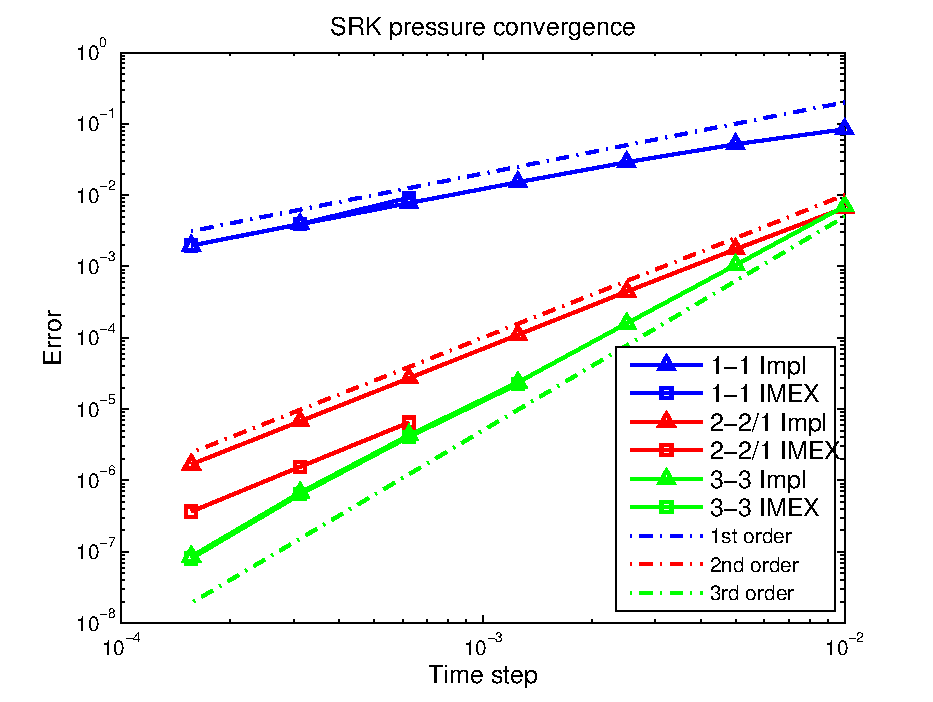
\includegraphics[width=0.49\textwidth]{Figures/Chapter6/cylinder/pre_impl_expl}}
  \caption{Fully implicit and IMEX-SRK convergence rate comparison.}
  \label{fig:IMEX_RK_cyl_conv_impl_expl}
\end{figure}
Fig. \ref{fig:IMEX_RK_cyl_conv_impl_expl} shows that the \textit{(3-3)} scheme is the most accurate one. Apart from the \textit{(2-2/1)} scheme, implicit and explicit versions give similar results when the time step is sufficiently small. 

Next, we look at the overall computational time needed for each approach. This is shown in Fig. \ref{fig:IMEX_RK_cyl_effi_impl_expl}, where the error $e_u$ is plotted against the CPU time for each scheme and for each approach.
\begin{figure}[h!]
  \centering
  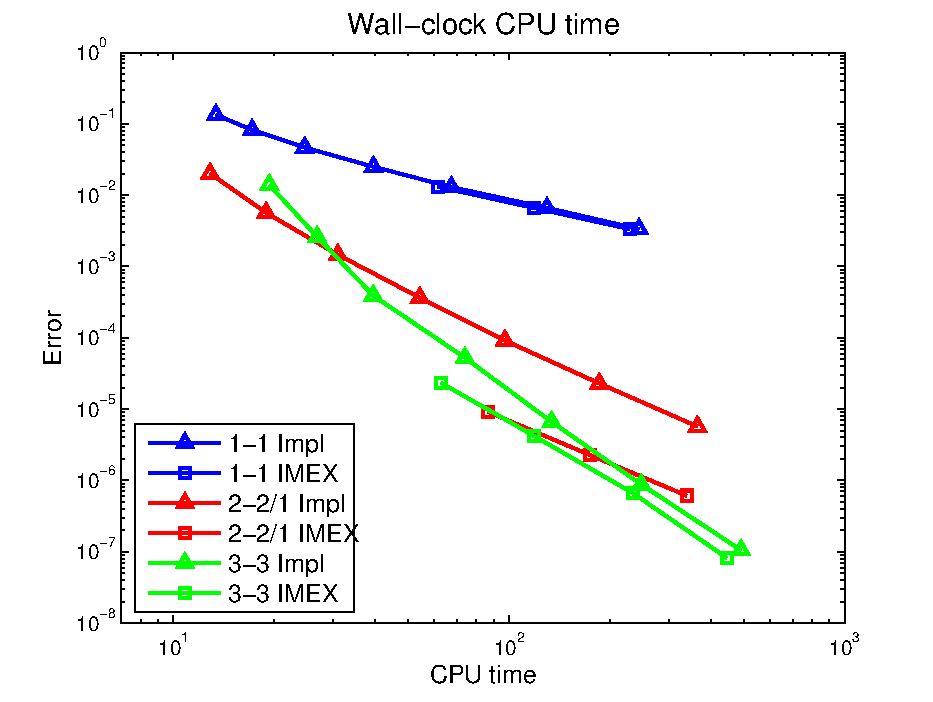
\includegraphics[width=0.49\textwidth]{Figures/Chapter6/cylinder/Efficiency_impl_expl}  
  \caption{Fully implicit and IMEX-SRK CPU time efficiency comparison.}
  \label{fig:IMEX_RK_cyl_effi_impl_expl}
\end{figure}
We see that, as expected, the approach with explicit time integration of the convective term is more efficient than the implicit one when the time step is sufficiently small. For large time steps, we cannot use the explicit versions since the ${\rm CFL}_u$ condition is limiting the stability of the method, and therefore its accuracy. Note that there is not a big difference on the efficiency for \textit{(1-1)} and \textit{(3-3)} schemes, since the gain of treating the convective term explicitly is not too much relevant in laminar problem types. As exposed at the beginning of this subsection, explicit approaches involve time step size restrictions, which may be much smaller than the physical time scale. Furthermore, as it has also been exposed before, the nonlinearity of the convective term when it is integrated implicitly does not increase the cost too much. Despite of that, for errors smaller than $\sim10^{-4}$, the most efficient scheme is the \textit{(3-3)} using explicit time integration of the convective term, at least for this test.

\subsubsection{Adaptive time stepping technique}
When solving generic transient flow problems, it is very useful to use an adaptive time stepping technique that will automatically provide a (dynamic) value of the time step size for a target accuracy. Time stepping techniques allow us to adapt the time step size to the flow conditions, that is to change the time step when the physical scales of the flow change, e.g., transition to turbulence. Adaptive time-stepping techniques have been implemented to satisfy accuracy requirements for the incompressible Navier-Stokes equations and several successful tests can be found in the literature, as it can be shown in \cite{feng_time-adaptive_2000,john_adaptive_2010,kay_adaptive_2010,veneziani_aladins:_2013}. 

These adaptive time stepping techniques can straightforwardly be applied to SRK methods. In fact, for all multi-step or multi-stage methods like SRK schemes, the implementation of an adaptive time step technique is widely used, since we only need a different evaluation of the final unknown at each step that can be done using a different Butcher tableau, see for instance \cite{gustafsson_control_1991,gustafsson_control-theoretic_1994}. Here we use the so called \textit{PI11 controller} by \cite{soderlind_automatic_2002} and suggested in \cite{gustafsson_control-theoretic_1994}, which computes the time step size as follows
$$\delta t_{n+1}=\left(\frac{\epsilon}{r_{n+1}}\right)^{1/k}\left(\frac{r_n}{r_{n+1}}\right)^{1/k}\frac{\delta t_n}{\delta t_{n+1}}\delta t_n,$$
with $\epsilon=0.8\cdot TOL$, where $TOL$ is a given tolerance that we take as $1\cdot10^{-6}$ and $0.8$ is a safety factor. The local error is $r_{n+1}=\|\U-\hat{\U}\|$ if the error per step (EPS) is controlled or $r_{n+1}=\|(\U-\hat{\U})/\delta t_n\|$ if the error per unit step (EPUS) is controlled. In the former case $k=p+1$ (EPS) and for the second one (EPUS) $k=p$, $p$ being the order of the time integration scheme which has been used to compute the estimated velocity $\hat{\U}$.

We solve the problem from $t=8.0$ to $t=8.4$ using the SRK \textit{(3-3)} scheme, considering the implicit time integration of the convective term. We compare the solutions against the one obtained with the same scheme, but using a fixed time step size $\delta t=3.125\cdot10^{-4}$, the smallest time step considered in previous analysis. Let us note that an adaptive time stepping technique for the explicit time integration of the convective term does not make sense in this case. We see in Table \ref{tab:CFLu_cyl} that the ${\rm CFL}_u$ number of the SRK with explicit versions of the convective term with a time step of $\delta t=3.125\cdot10^{-4}$ is already above the critical value of $1.0$. This means that if we increase the time step size, we will have stability problems due to the hyperbolic ${\rm CFL}$ condition. 

To compute $\hat{\U}$ we have used the 2nd order Butcher tableau referred as \textit{Embedded Formula of Order 2} for the \textit{Third Order Strongly S-Stable Formula} defined in \cite{cash_diagonally_1979}, which is 3rd order and
%The Butcher tableau used to compute $\hat{\U}$ is the \textit{Embedded Formula of Order 2} for the \textit{Third Order Strongly S-Stable Formula} defined in \cite{cash_diagonally_1979}, which 
corresponds to the \textit{(3-3)} scheme defined in \ref{appendix:Butcher_tab}. The initial time step size is set to be $\delta t_0=1.0\cdot10^{-5}$, small enough to get an accurate first solution. In Fig. \ref{fig:IMEX_RK_cyl_adp_dt} we show the time step evolution for the two different cases considered in this subsection. We see that the time step size for the scheme with adaptive time stepping is increasing with a variable rate and seems to converge to an optimal one. %evolving  following a shape which is directly related to the flow performance.
\begin{figure}[h!]
  \centering
  \subfigure[Time step evolution]{\label{fig:IMEX_RK_cyl_adp_dt}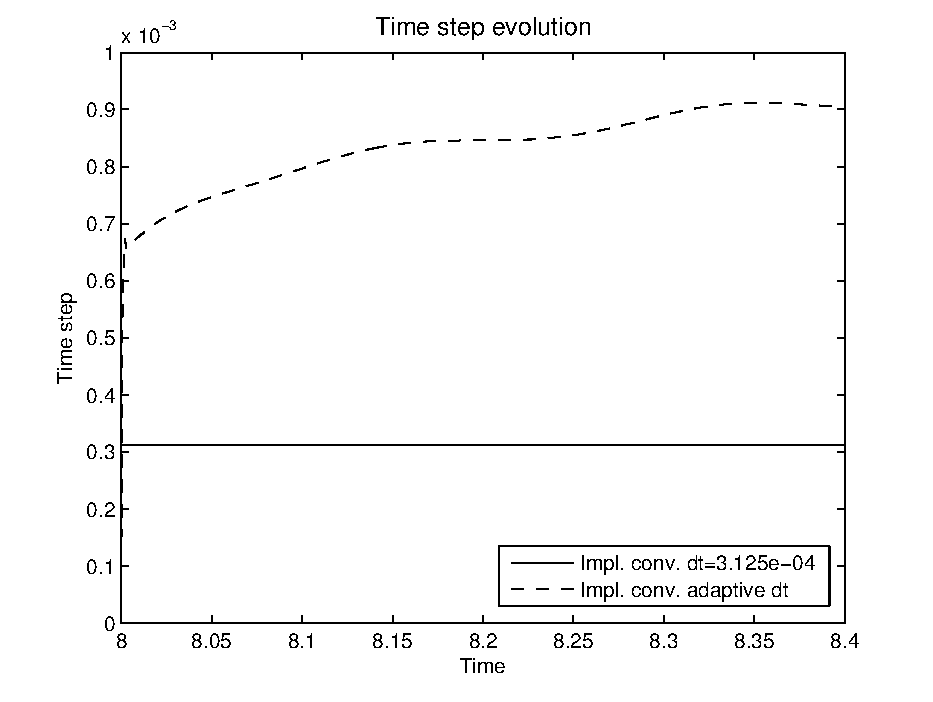
\includegraphics[width=0.49\textwidth]{Figures/Chapter6/cylinder/time_step}}    
  \subfigure[Lift coefficient (close up view)]{\label{fig:IMEX_RK_cyl_adp_lift}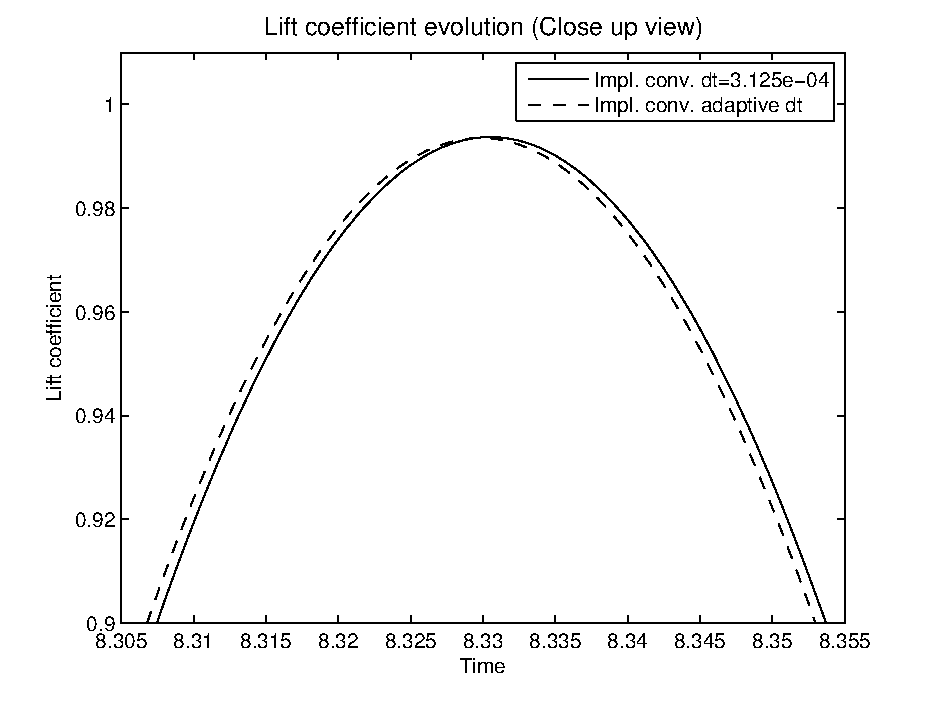
\includegraphics[width=0.49\textwidth]{Figures/Chapter6/cylinder/lift_close}}
  \caption{Adaptive time stepping.}
  \label{fig:IMEX_RK_cyl_adp}
\end{figure}
Fig. \ref{fig:IMEX_RK_cyl_adp_lift} depicts a close up view of the lift coefficient evolution. We see that for the implicit adaptive time step case, the results are really close to those obtained with the same scheme with a fixed time step of $\delta t=3.125\cdot10^{-4}$. Note that the adaptive time step size are twice or even three times larger than the fixed one. The total elapsed CPU time for the implicit scheme with adaptive time step is $3615$ s, while the total time for the implicit scheme with fixed time step is $8453$ s, which supposes a reduction of a $42.8\%$ of time consumption with a very little difference in the result.

\subsection{Taylor-Green vortex flow}
\label{subsec-C6_TGV}
The next step of this work is to check the performance of the SRK methods for turbulent incompressible flows. The use of IMEX-SRK methods is usually favoured for turbulent flows, since the time step size required to satisfy the  ${\rm CFL}_u$ condition is of the same order as the physical one needed for accuracy purposes. 
%As it was said in Subsection \ref{subsec-C6_cylinder}, the efficiency of explicit or IMEX time integration schemes could be more significant in this kind of flows. %For unbounded turbulent flows, the physical time scale is very small, so we are forced to use small time steps in order to capture properly the physical phenomena. Then, here we could be interested in having more efficient solvers, although the presence of a critical time step size, since it may be of the order of the physical time scale.
The Taylor-Green vortex (TGV) problem is a typical and widely used problem in turbulence numerical simulations, in which we can see the basic turbulence decay mechanisms  in a relatively simple flow. Here, the computational domain is the cube $(0,2\pi)^3$ with periodical boundary conditions. The initial analytical condition for this problem is given by (see, e.g., \cite{brachet_direct_1991})
\begin{align}
\label{eq-C6_ini_sol_TG}
&\u(x,y,z,0)=\left(\begin{array}{c}
u_x\\
u_y\\
u_z
\end{array}\right)=\left(\begin{array}{c}
u_0\cos(x)\sin(y)\sin(z)\\
-u_0\sin(x)\cos(y)\sin(z)\\
0
\end{array}\right)\\\nonumber
&p(x,y,z,0)=p_0+\frac{1}{16}\left(\cos(2x)+\cos(2y)\right)\left(\cos(2z)+2\right),
\end{align}
with
$$u_0=\frac{2}{\sqrt{3}}\sin\left(\gamma+\frac{2\pi}{3}\right).$$
We choose $\gamma=0$, which gives the mean initial velocity  $u_0=1$. We solve the TGV problem using a Reynolds number ${\rm Re}=1600$, but in the literature the same test using different Reynolds numbers (e.g., ${\rm Re}=800$ and ${\rm Re}=3000$) can be found (see, e.g., \cite{gassner_accuracy_2013,hickel_adaptive_2006}).

The problem is solved in a $64^3$ $Q_2/Q_1$ elements mesh, and no additional sub-grid modelling is being used. Our concern is about the time integration, therefore the spatial accuracy does not take a crucial role in this work. Anyway, we analyze some physical quantities, like the global kinetic energy or the kinetic energy dissipation rate, that are typically used for this test to calibrate different methods.

We only use the IMEX-SRK method with the convection treated explicitly, avoiding the need of nonlinear iterations. This situation is given by defining the operators $\mathcal{F}$ and $\mathcal{G}$ in  Eqs. (\ref{eq-C6_IMEX_NS_up}) and \Eq{C6_IMEX_NS_up_n+1} as
$$\mathcal{F}(\U):=-K\U,\quad\quad\mbox{and}\quad\quad\mathcal{G}(\U,\P):=\F-C(\U)\U-G\P.$$

First of all, we perform a time step convergence analysis at the beginning of the simulation, where the flow is still laminar. This convergence analysis consists in solving the problem from $t=0.0$ to $t=0.1$ for all the schemes proposed in \ref{appendix:Butcher_tab} for several time step sizes. In particular, we solve the problem with four different time step sizes ($\delta t=\{0.1,0.05,0.025,0.0125\}$) and we compare the solution against the one obtained with the \textit{(5-3)} scheme with a time step equal to $\delta t=6.25\cdot10^{-3}$. The $L^2$-norm of the kinetic energy error compared against the reference kinetic energy solution given by a DNS computation can be found in  \cite{boom_time-accurate_????}. Our approach is to compute the $L^{\infty}$-norm of the solution, comparing against a solution computed with a finer time step, but with the same spatial discretization. With this approach we are eliminating the spatial error and we are using a more restrictive error norm.

We show in Fig. \ref{fig:TGV_conv_laminar} the order of convergence in time for both velocity (Fig. \ref{fig:TGV_vel_laminar}) and pressure (Fig. \ref{fig:TGV_pre_laminar}) fields. We can see that the order of convergence in this regime follows the predicted rate for almost all schemes; the \textit{(5-3)} schemes seems to converge with a higher rate than the expected one, being this performance especially remarkable for the velocity field convergence.

\begin{figure}[h!]
  \centering
  \subfigure[Velocity]{\label{fig:TGV_vel_laminar}\includegraphics[width=0.49\textwidth]{Figures/Chapter6/TGV/imex_nsi_explcnv_64_vel_T0_Re1600_dt6dot25e-3}}    
  \subfigure[Pressure]{\label{fig:TGV_pre_laminar}\includegraphics[width=0.49\textwidth]{Figures/Chapter6/TGV/imex_nsi_explcnv_64_pre_T0_Re1600_dt6dot25e-3}}
  \caption{IMEX-SRK convergence for the laminar regime.}
  \label{fig:TGV_conv_laminar}
\end{figure}

Another point to be highlighted in Fig. \ref{fig:TGV_conv_laminar} is that the \textit{(2-2/1)} scheme shows a much lower error compared to the other second-order schemes. This performance is also observed on the previous tests when an IMEX-SRK (with explicit treatment of the convection) is used. 

As it has been done for the 2D laminar flow around a cylinder test (see Subsection \ref{subsec-C6_cylinder}) we analyze the efficiency of the methods comparing error  against CPU time. This comparison is in  Fig. \ref{fig:TGV_effi_laminar}, where the error is plotted in terms of the averaged elapsed CPU time per processor needed to complete the simulation from $t=0$ to $t=0.1$.

\begin{figure}[h!]
  \centering
  \includegraphics[width=0.49\textwidth]{Figures/Chapter6/TGV/imex_nsi_explcnv_64_T0_Re1600_dt6dot25e-3_effi}
  \caption{IMEX-SRK efficiency for the laminar regime.}
  \label{fig:TGV_effi_laminar}
\end{figure}
It is seen in Fig. \ref{fig:TGV_effi_laminar} that the most efficient schemes are the \textit{(2-2/1)} and  \textit{(3-3)} ones, which for errors greater than $\sim10^{-6}$ give the same error-CPU time ratio. As it is natural, below this threshold, the second-order scheme \textit{(2-2/1)} starts loosing efficiency and the \textit{(3-3)} scheme becomes the most efficient one for errors smaller than $\sim10^{-6}$.

Once we have determined that the most efficient schemes for this test are the \textit{(2-2/1)} and \textit{(3-3)} ones, we now want to see their performance for a larger time interval. The aim is to solve the problem until the turbulence becomes fully developed, which for this Reynolds number case takes place around $t\sim9$. Following \cite{brachet_direct_1991}, the time interval will go from $t=0.0$ to $T=10.0$, so we will be able to compare the results with their DNS. For this computation, we select the time step size that has an error at $t=0.1$ in Fig. \ref{fig:TGV_vel_laminar} of the order $\sim1\cdot10^{-6}$, i.e., $\delta t=5.0\cdot10^{-2}$ for the \textit{(3-3)} scheme and $\delta t=3.6\cdot10^{-2}$ for the \textit{(2-2/1)} scheme.

Fig. \ref{fig:TGV_ene_ens} depicts the total energy evolution (Fig. \ref{fig:TGV_ene}) and the kinetic energy dissipation rate of the resolved scales (Fig. \ref{fig:TGV_ens}) compared against the DNS provided by \cite{brachet_direct_1991}. The result is exactly the same for both schemes, despite the fact that the third-order scheme uses a larger time step. Looking at Fig. \ref{fig:TGV_ene}, we see that the energy evolution of the solution is not far from the DNS, but there is a gap after $t=6$, when the turbulence is developed. This is caused by the lack of any turbulent model which would capture the small scales proper dissipation. For the same reason we see big differences between our solutions and the DNS results in Fig. \ref{fig:TGV_ens} after $t=6$.

\begin{figure}[h!]
  \centering
  \subfigure[Global energy.]{\label{fig:TGV_ene}\includegraphics[width=0.49\textwidth]{Figures/Chapter6/TGV/imex_nsi_explcnv_64_ene}}    
  \subfigure[Kinetic energy dissipation rate.]{\label{fig:TGV_ens}\includegraphics[width=0.49\textwidth]{Figures/Chapter6/TGV/imex_nsi_explcnv_64_ens}}
  \caption{Global energy and Kinetic energy dissipation rate evolution (blue line below red line).}
  \label{fig:TGV_ene_ens}
\end{figure}

Looking at Fig. \ref{fig:TGV_ens} we clearly see that the error given by the spatial discretization when the flow becomes turbulent is too large to appreciate significant differences between time integration schemes. We want to highlight here that an adaptive time step technique could be used in order to efficiently solve the transient problem. However, the use of an adaptive time stepping technique without an accurate solution in space does not make sense. Future work in this direction involves the introduction of LES models within the IMEX-SRK approach proposed in this work.

%The efficiency in terms of computational time of both schemes for the laminar regime is shown in Fig. \ref{fig:TGV_effi_laminar}, where we see that for an error in time less than $1.0\cdot10^{-5}$, the \textit{(5-3)} scheme is much more efficient than the \textit{(1-2)} one, although this last one requires less stages on the computation. The time shown in Fig. \ref{fig:TGV_effi_laminar} is given in seconds and corresponds to the averaged total elapsed time per processor needed to complete the simulation from $t=0$ to $t=0.1$.

%For this test we only use two different Butcher tableau definitions: one is the \textit{(1-2)}, equivalent to the Crank-Nicolson scheme, and the other one is the \textit{(5-3)}. Initially we solve the problem from $t_0=0$ to $T=10$ for both schemes only for the Half-IMEX Runge-Kutta method with the convection treated explicitly, avoiding the need of nonlinear iterations. This situation is given by defining the operators $\mathcal{F}$ and $\mathcal{G}$ in (\ref{eq-C6_NS_galerkin_mat1_ope}) as
%$$\mathcal{F}(\U):=-K\U,\quad\quad\mbox{and}\quad\quad\mathcal{G}(\U,\P):=\F-C(\U)\U-G\P.$$
%
%The time step size for the \textit{(1-2)} scheme is set $\delta t=7.5\cdot10^{-3}$ and $\delta t=2.5\cdot10^{-2}$ for the \textit{(5-3)} scheme, more than 3 times larger. The justification of this choice is given below.
%
%Fig. \ref{fig:TGV_ene_ens} depicts the total energy evolution (Fig. \ref{fig:TGV_ene}) and the kinetic energy dissipation rate of the resolved scales (Fig. \ref{fig:TGV_ens}) compared against the DNS provided by \cite{brachet_direct_1991}. It is seen that the result is exactly the same for both schemes, despite the third-order scheme uses a time step more than 3 times largest. Looking at Fig. \ref{fig:TGV_ene} we see that the energy evolution of the solution is not far from the DNS, but there is a gap after $t=6$, when the turbulence is developed. This is caused by the lack of any turbulent model which would capture the small scales proper dissipation. For the same reason we see big differences between our solutions and the DNS results in Fig. \ref{fig:TGV_ens} after $t=6$.
%
%\begin{figure}[h!]
%  \centering
%  \subfigure[Global energy.]{\label{fig:TGV_ene}\includegraphics[width=0.49\textwidth]{Figures/TGV/imex_nsi_explcnv_64_ene}}    
%  \subfigure[Kinetic energy dissipation rate.]{\label{fig:TGV_ens}\includegraphics[width=0.49\textwidth]{Figures/TGV/imex_nsi_explcnv_64_ens}}
%  \caption{Global energy and Kinetic energy dissipation rate evolution.}
%  \label{fig:TGV_ene_ens}
%\end{figure}
%
%Now we perform a time step convergence analysis for both schemes for $t\in[0,0.1]$, where the flow is still laminar, and for $t\in[8,8.1]$, where the flow is turbulent. To do that we solve the problem from with 4 different time step sizes ($\delta t=\{0.1,0.05,0.025,0.0125\}$) and we compare the solution against the one obtained with the \textit{(5-3)} scheme with a time step equal to $\delta t=6.25\cdot10^{-3}$. Here, \cite{boom_time-accurate_????} computes the $L^2$-norm of the kinetic energy error comparing against the reference kinetic energy solution given by a DNS computation. Our approach is to compute the $L^{\infty}$-norm of the solution, comparing against a solution computed with a finer time step, but with the same spatial discretization. With this approach we are eliminating the spatial error and we are using a more restrictive error norm.
%
%\subsubsection{Laminar regime}
%
%\begin{figure}[h!]
%  \centering
%  \subfigure[Velocity]{\label{fig:TGV_vel_laminar}\includegraphics[width=0.49\textwidth]{Figures/TGV/imex_nsi_explcnv_64_vel_T0_Re1600_dt6dot25e-3}}    
%  \subfigure[Pressure]{\label{fig:TGV_pre_laminar}\includegraphics[width=0.49\textwidth]{Figures/TGV/imex_nsi_explcnv_64_pre_T0_Re1600_dt6dot25e-3}}
%  \caption{IMEX-RK convergence for the laminar regime.}
%  \label{fig:TGV_conv_laminar}
%\end{figure}
%
%In Fig. \ref{fig:TGV_conv_laminar} we show the order of convergence in time for both velocity (Fig. \ref{fig:TGV_vel_laminar}) and pressure (Fig. \ref{fig:TGV_pre_laminar}) fields. We can see in Fig. \ref{fig:TGV_conv_laminar} that the order of convergence in this regime for the third order scheme is even greater than the one predicted by the Butcher tableau definition. Moreover, here comes the reason of the choice of different time step sizes for the computation of the full simulation that was exposed before. Given a time step of the $\delta t=7.25\cdot10^{-3}$ for the \textit{(1-2)} scheme, making a simple extrapolation from Fig. \ref{fig:TGV_conv_laminar} the time step for the \textit{(5-3)} that gives more or less the same error is $\delta t=2.5\cdot10^{-2}$.
%
%\begin{figure}[h!]
%  \centering
%  \includegraphics[width=0.49\textwidth]{Figures/TGV/imex_nsi_explcnv_64_T0_Re1600_dt6dot25e-3_effi}
%  \caption{IMEX-RK efficiency for the laminar regime.}
%  \label{fig:TGV_effi_laminar}
%\end{figure}
%
%The efficiency in terms of computational time of both schemes for the laminar regime is shown in Fig. \ref{fig:TGV_effi_laminar}, where we see that for an error in time less than $1.0\cdot10^{-5}$, the \textit{(5-3)} scheme is much more efficient than the \textit{(1-2)} one, although this last one requires less stages on the computation. The time shown in Fig. \ref{fig:TGV_effi_laminar} is given in seconds and corresponds to the averaged total elapsed time per processor needed to complete the simulation from $t=0$ to $t=0.1$.
%
%\subsubsection{Turbulent regime}
%
%At $t=8.0$ the turbulence is fully developed as it is seen at Fig. \ref{fig:TGV_ens}, where at that time the energy dissipation rate is near to reach its maximum value. So at this point we can evaluate the performance of the proposed integration schemes in a turbulent regime.
%
%In Fig. \ref{fig:TGV_conv_turbulent} we show the convergence in time of \textit{(1-2)} and \textit{(5-3)} schemes. Similar order of convergence is achieved in the turbulent regime, compared with the laminar case shown before. The order of convergence does not seem to be affected by the flow state, but the absolute value of the error does. Looking at the velocity (Fig. \ref{fig:TGV_vel_turbulent}) and the pressure (Fig. \ref{fig:TGV_pre_turbulent}) error values, we see that they are about four orders of magnitude higher than the ones in the laminar regime. As it is natural, we expect a greater error in time for a more fluctuating flow. This result also indicates that the temporal scale is much lower for the turbulent regime than the laminar case. Therefore, as exposed in subsection \ref{subsec-C6_cylinder}, in this kind of flows the critical time step is not given by stability requirements, but by the temporal scale of the flow which will affect the accuracy of the solution.
%
%\begin{figure}[h!]
%  \centering
%  \subfigure[Velocity]{\label{fig:TGV_vel_turbulent}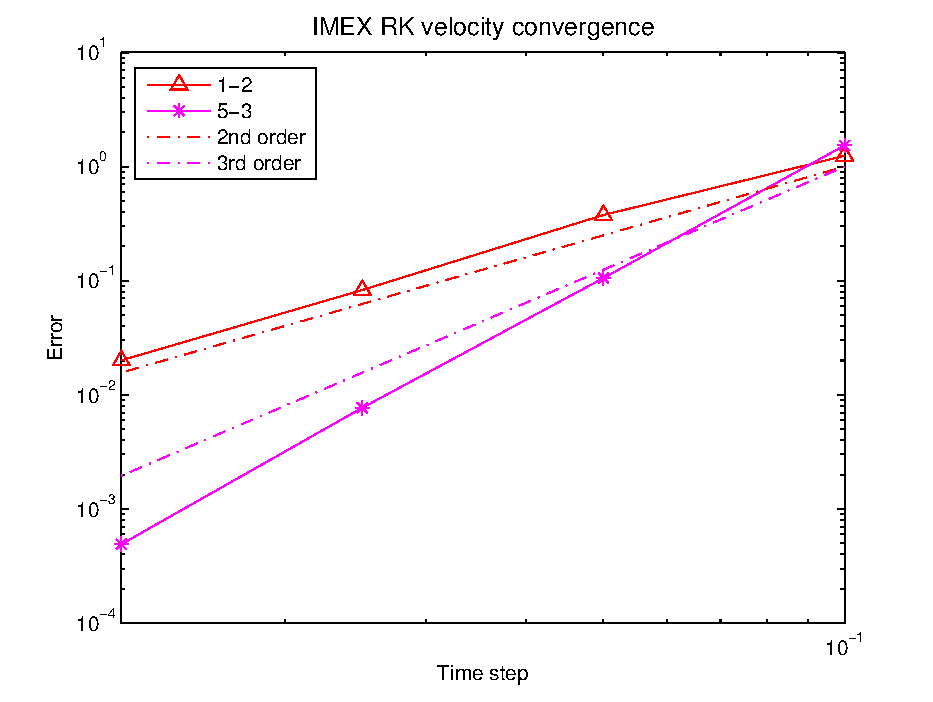
\includegraphics[width=0.49\textwidth]{Figures/TGV/imex_nsi_explcnv_64_vel_T8_Re1600_dt6dot25e-3}}    
%  \subfigure[Pressure]{\label{fig:TGV_pre_turbulent}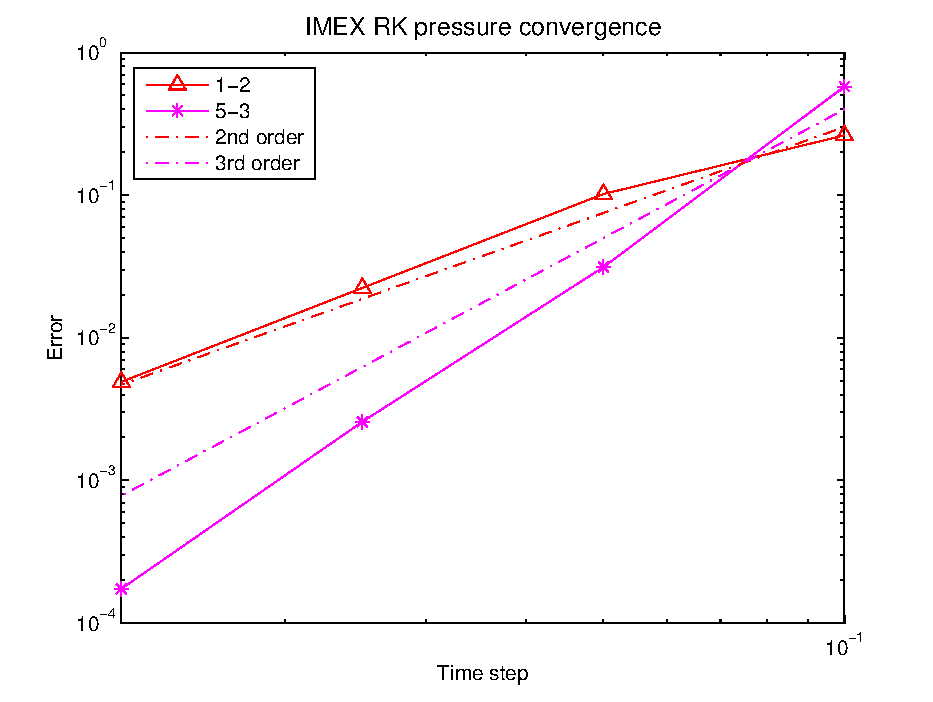
\includegraphics[width=0.49\textwidth]{Figures/TGV/imex_nsi_explcnv_64_pre_T8_Re1600_dt6dot25e-3}}
%  \caption{IMEX-RK convergence for the turbulent regime.}
%  \label{fig:TGV_conv_turbulent}
%\end{figure}
%
%In terms of computational efficiency, Fig. \ref{fig:TGV_effi_turbulent} shows that the gain in efficiency of the \textit{(5-3)} scheme that appeared in the laminar regime is not so clear here. In this case, both curves tend to be more parallel and the intersection between them (indicated by the tendency of the \textit{(1-2)} curve) seems to be for higher CPU times. However, since the error in this figure is larger than in Fig. \ref{fig:TGV_effi_laminar} it could be said that if we are looking for errors in time of the order of $10^{-2}$, the \textit{(5-3)} is the most efficient time integration scheme.
%
%\begin{figure}[h!]
%  \centering
%  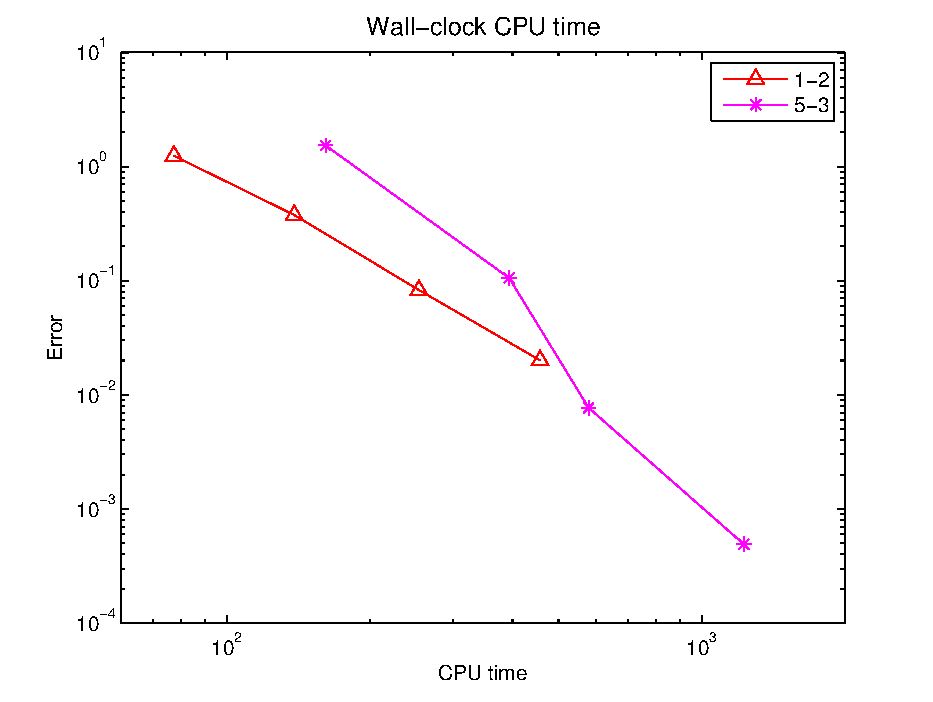
\includegraphics[width=0.49\textwidth]{Figures/TGV/imex_nsi_explcnv_64_T8_Re1600_dt6dot25e-3_effi}
%  \caption{IMEX-RK efficiency for the turbulent regime.}
%  \label{fig:TGV_effi_turbulent}
%\end{figure}
%
%A very clear result that can be observed comparing the results for the TGV test in the laminar regime and the turbulent one is that, if we want to keep the same order of the error in time, an adaptive time step technique must be used. In this type of problems, where there is a transition between laminar to turbulent flow, there may be a large difference in the temporal scales. Then, in order to guarantee accurate results, the time step size has to be adapted to them.
%
%Adaptive time-stepping techniques have been implemented to satisfy accuracy requirements for the incompressible Navier-Stokes equations and several successful tests can be found in the literature, as it can be shown in \cite{feng_time-adaptive_2000,john_adaptive_2010,kay_adaptive_2010,veneziani_aladins:_2013}.
%
%These adaptive time step techniques are quite direct to be implemented in the Half-IMEX Runge-Kutta method. In fact, for all multi-step or multi-stage methods like the Runge-Kutta schemes, the implementation of an adaptive time step technique is widely used since we only need a different evaluation of the final unknown at each step that can be done using a different Butcher tableau, see for instance \cite{gustafsson_control_1991,gustafsson_control-theoretic_1994}.

\section{Conclusions}
\label{sec-C6_conclusions}

The segregated Runge-Kutta methods proposed in this work enjoy two nice features, namely the velocity and pressure segregation at the time integration level (without the need to perform additional fractional step techniques that spoil high orders of accuracy) and the provable same order of accuracy for both velocities and pressures. These methods have been motivated as an implicit-explicit Runge-Kutta time integration of the projected Navier-Stokes system onto the discrete divergence-free space. The terms in this system that involve the inverse of a discrete Laplacian $\D\M^{-1} G$ are treated explicitly in all cases, in order to make the resulting method numerically feasible. Viscous and convection terms can be treated using implicit, combined implicit/explicit, or fully explicit schemes, leading to implicit, IMEX, or explicit SRK schemes, respectively. The pressure can be recovered by using a discrete pressure Poisson equation, and the SRK scheme can be finally recasted in a velocity-pressure formulation.

Explicit SRK methods have been proved to be equivalent to existing half-explicit RK methods. Further, these methods exactly satisfy the divergence-constraint equation in most situations of interest; in all cases when weakly enforcing Dirichlet boundary conditions, and for fixed or at most a point-wise $p$-th order polynomial variation in time (for a $p$-th order method) of the Dirichlet data for a strong enforcement. Further, it is easy to check that the error for the pressure is of the same order as the one for the velocity.

We have performed a wide set of numerical experiments to evaluate the segregated Runge-Kutta algorithms; first to third order schemes have been implemented and analyzed. They include convergence tests for problems with  manufactured solutions for time-dependent Dirichlet boundary data. This way, we can also evaluate the well-known order reduction effect of RK methods. We have also performed numerical tests for the laminar flow around a cylinder (evaluating drag and lift coefficients) and the turbulent Taylor-Green vortex flow. The different methods have been compared in terms of CPU cost for a target error. Fully implicit, implicit viscous/explicit convective, and fully explicit methods have been evaluated, considering their respective CFL conditions. Fully implicit SRK schemes have shown a remarkably strong stability and high accuracy till about 100 times the explicit CFL condition. Further, segregated Runge-Kutta schemes with adaptive time stepping have been proposed and analyzed numerically. 

The use of SRK schemes is very appealing for large scale computations of incompressible flows, since the monolithic indefinite system is replaced by segregated positive-definite velocity and pressure blocks. The pressure block involves a Poisson solver, whereas the velocity block is a vector-Laplacian or elasticity matrix when the convective term is treated explicitly. Massively parallel solvers for these problems can be found in the literature (see, e.g., \cite{art003}) and are at the user's disposal, e.g., within the FEMPAR scientific computing software.